\section{Simulación de la propagación}

El presente experimento busca analizar la propagación del fuego. Una opción para simularlo pudiera ser mediante la definición manual de la regla que gobierne el sistema. Por ejemplo, podemos definir tres estados: vivo, quemado y quemándose, en donde toda célula viva que tenga un vecino quemándose se quema en el siguiente paso, y toda célula quemándose se apaga. Si bien esta definición podría mostrar dinámicas de propagación, no está definida mediante un sistema real, objetivo de esta investigación.

Este experimento se alimenta del conjunto de datos FLAME~3 \cite{hopkins2024flame3datasetunleashing}, que captura la quema de Hanna Hammock en 2023. Sus autores utilizaron un dron que captura imágenes térmicas con vista cenital\footnote{Cenit: punto más alto en el cielo, ubicado a 90° por encima del observador \cite{plano_cenital}.} para la gestión de incendios forestales. Este conjunto de datos contiene tres carpetas de imágenes: en formato ``tiff'', que registran la temperatura, en ``jpg'' con vista térmica y en ``jpg'' regular.

\subsection{Preprocesamiento de los datos}

Para la limpieza del conjunto de datos, se procedió de la siguiente manera: 

\begin{enumerate}
	\item Selección de conjuntos de mayor representación: El conjunto de datos completo contiene la vista de tres diferentes zonas, de las cuales solo los \textit{plot} 1 y 2 contienen la secuencia en formato ``tiff'' durante la quema. De estos conjuntos, se consideran las siguientes dos particiones como representantes de la propagación:

	\begin{itemize}
		\item flame\_plot\_1 (\textit{plot} 1 de Kaggle): de la imagen 662 a la 777, 116 \textit{frames}
		\item flame\_plot\_2 (\textit{plot} 2 de Kaggle): de la imagen 1189 a la 1254, 66 \textit{frames}
	\end{itemize}
	
	Estos rangos se caracterizan por mostrar la propagación del fuego de un $\sim 2\%$ a un $\sim 86\%$ del espacio en flame\_plot\_1 y de un $\sim 4\%$ a casi el $100\%$ en flame\_plot\_2. Iniciar con fuego dentro del sistema es esencial para que la red neuronal no infiera combustión espontánea. Además, se seleccionan estos rangos por ser los que incluyen una propagación con velocidad constante. 

	\item Ajuste de posición: El dron se mueve por el viento, por lo que un desajuste de varios píxeles obliga a incrementar la vecindad en cada dirección para capturar el error. Para esto, se opta por la siguiente técnica que ajusta la imagen:

	\begin{enumerate}
		\item Se mide el desplazamiento entre pares de imágenes mediante correlación de fase con precisión de $1/20$ de píxel. Para que el movimiento del fuego no se confunda con el movimiento de la cámara, solo se compara la textura del suelo frío (menos de 50 °C en ambas imágenes y a más de 12 píxeles del fuego).
		\item Cada imagen se compara no solo con la siguiente, sino con las que están a 1, 2, 4, 8, \dots, 128 imágenes de distancia. Al encadenar únicamente imágenes consecutivas, el error de cada medición se acumula a lo largo de la secuencia.
		\item Con todas las mediciones se resuelve la posición de cada imagen respecto a la primera mediante mínimos cuadrados robustos (pérdida de Huber), lo que reduce el peso de las mediciones erróneas.
		\item Cada imagen se desplaza a la posición de la primera mediante interpolación bilineal. La corrección máxima fue de 6.57 píxeles en flame\_plot\_1 y de 7.69 píxeles en flame\_plot\_2.
	\end{enumerate}

	Sin embargo, las imágenes resultantes generan bordes negros que representan el movimiento de la imagen. Esto genera ruido en los bordes, lo que nos obliga a reducir el tamaño de los datos.
	
	\item Eliminación de ruido residual: Al desplazar cada imagen, la zona que queda fuera de la imagen original se rellena con píxeles negros (sin dato). Para ello, se extrae de la imagen el cuadrado de mayor tamaño que no tenga ruido en ninguna imagen de la secuencia (esto para ambas secuencias), y se obtiene la imagen reducida, tal como se muestra en la figura \ref{fig:experimentacion:natuales:Flame3:clean_03}.
	
	\item Escalado de la evolución: Con la imagen reducida, se aplican operaciones de convolución con el objetivo de reducir el tamaño de la imagen a $100 \times 100$ píxeles y disminuir la complejidad de la dinámica. Sin embargo, este método reduce el conjunto de entrenamiento, porque disminuye la cantidad de vecindades que podemos extraer. 
	
	 \item Discretización: El objetivo de este experimento es simular la propagación del fuego y no la propagación de la temperatura. Estos datos están estrechamente relacionados, pero si únicamente consideramos los registros de temperatura, ignoramos que el fuego no se puede propagar dos veces por el mismo terreno. Es por esto que el sistema debe conocer cuándo hay un incendio y distinguir si los registros corresponden a su temperatura antes o después del fuego. 
	 
	 Para resolver esto, se discretizan los píxeles y se ajustan a 18 estados según las temperaturas de la tabla \ref{tab:flame_states_proportion}. Los estados $ \mathcal{S}_b = \{0, 1, \dots, 11\}$ corresponden a las temperaturas normales y su incremento conforme el fuego se propaga y la temperatura aumenta, mientras que los estados $\mathcal{S}_t = \{12, 13, \dots, 17\}$ corresponden al enfriamiento del sistema. Sea $\tau_{\vec{i}}(t) \in \{0, 1, \dots, 11\}$ el estado de temperatura de la célula $\vec{i}$, $T_{\vec{i}}(t)$ su temperatura en °C y $m_{\vec{i}}$ la temperatura mínima que ha registrado desde que se quemó. Definimos la siguiente regla para asignar los estados:
	 \[
	 	\sigma_{\vec{i}}(t + 1) \in
	 	\begin{cases}
	 		\mathcal{S}_t & \text{si } \tau_{\vec{i}}(t + 1) < \tau_{\vec{i}}(t) \\
	 		\mathcal{S}_b & \text{si } \sigma_{\vec{i}}(t) \in \mathcal{S}_t,\ T_{\vec{i}}(t + 1) > m_{\vec{i}} + 30\,^\circ\mathrm{C} \\
	 		\text{el de } \sigma_{\vec{i}}(t) & \text{en otro caso}
	 	\end{cases}
	 \]
	 donde una célula en $\mathcal{S}_b$ toma el estado $\tau_{\vec{i}}(t + 1)$ y una en $\mathcal{S}_t$ toma el estado $12 + \lfloor \tau_{\vec{i}}(t + 1) / 2 \rfloor$, por lo que los estados quemados agrupan las temperaturas de dos en dos.

	 Es decir, si se enfría pasa a un estado quemado, pero si su temperatura aumenta nuevamente más de 30 °C sobre el mínimo registrado desde que se quemó, deja de estar quemada y regresa a su estado de temperatura.
	 
\end{enumerate}

\begin{table}[htbp]
	\centering
	\footnotesize
	\begin{tabular}{ccccc}
		\toprule
		& & & \textbf{Porcentaje en} & \textbf{Porcentaje en} \\
		\textbf{Estado} & \textbf{Tipo} & \textbf{Temperatura} & \textbf{flame\_plot\_1} & \textbf{flame\_plot\_2} \\ \midrule
		0 & \multirow{12}{*}{Temperatura} & 25.3--59.0 & 49.13 & 16.74 \\
		1 &  & 59.0--72.9 & 1.45 & 4.07 \\
		2 &  & 72.9--90.1 & 0.87 & 2.25 \\
		3 &  & 90.1--111.4 & 0.77 & 1.35 \\
		4 &  & 111.4--137.6 & 0.76 & 1.15 \\
		5 &  & 137.6--170.0 & 0.70 & 1.11 \\
		6 &  & 170.0--210.0 & 0.71 & 1.10 \\
		7 &  & 210.0--259.5 & 0.74 & 1.25 \\
		8 &  & 259.5--320.6 & 0.83 & 1.43 \\
		9 &  & 320.6--396.1 & 0.82 & 1.92 \\
		10 &  & 396.1--489.3 & 0.15 & 2.13 \\
		11 &  & 489.3--604.6 & 0.00 & 0.28 \\ \midrule
		12 & \multirow{6}{*}{Quemado} & 25.3--72.9 & 23.82 & 10.79 \\
		13 &  & 72.9--111.4 & 9.24 & 15.88 \\
		14 &  & 111.4--170.0 & 5.72 & 16.59 \\
		15 &  & 170.0--259.5 & 3.25 & 13.34 \\
		16 &  & 259.5--396.1 & 1.03 & 7.81 \\
		17 &  & 396.1--604.6 & 0.01 & 0.80 \\ \bottomrule
	\end{tabular}
	\caption{Estados de FLAME~3 con 12 estados de temperatura y 6 de quemado, su rango de temperatura en °C y el porcentaje de células en cada estado.}
	\label{tab:flame_states_proportion}
\end{table}

	El resultado se muestra en la figura \ref{fig:flame_clean_process}, que presenta la conversión de una imagen durante cada uno de los pasos ya mencionados. Cabe mencionar que este proceso no se realiza sobre las imágenes ``jpg'', sino sobre las ``tiff'', ya que las primeras ajustan los colores según los rangos de temperatura presentes, por lo que dos temperaturas pueden tener el mismo color asociado en diferentes imágenes, mientras que las ``tiff'' almacenan la temperatura de cada posición.
	
	\begin{figure}[htbp]
		\centering
		\begin{subfigure}[b]{0.35\textwidth}
			\centering
			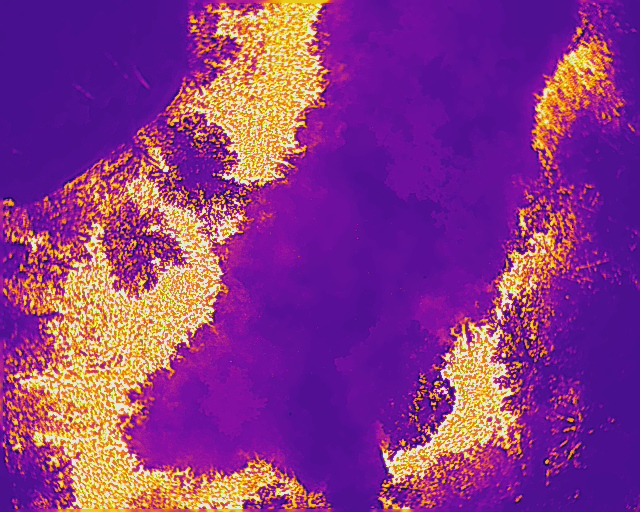
\includegraphics[width=\linewidth]{img/experimentacion/naturales/Flame3/clean_01.jpg}
			\caption{Imagen original}
			\label{fig:experimentacion:natuales:Flame3:clean_01}
		\end{subfigure}
		\hfill 
		\begin{subfigure}[b]{0.35\textwidth}
			\centering
			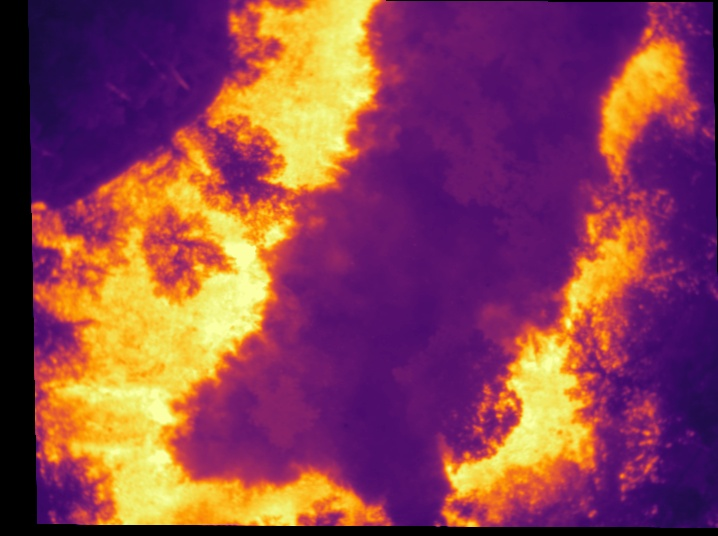
\includegraphics[width=\linewidth]{img/experimentacion/naturales/Flame3/clean_02.jpg}
			\caption{Ajuste de posición}
			\label{fig:experimentacion:natuales:Flame3:clean_02}
		\end{subfigure}
		\hfill 
		\begin{subfigure}[b]{0.30\textwidth}
			\centering
			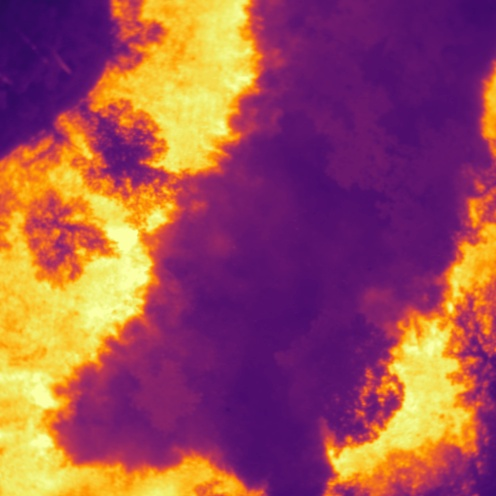
\includegraphics[width=0.75\linewidth]{img/experimentacion/naturales/Flame3/clean_03.jpg}
			\caption{Eliminación de ruido residual}
			\label{fig:experimentacion:natuales:Flame3:clean_03}
		\end{subfigure}
		\hfill 
		\begin{subfigure}[b]{0.30\textwidth}
			\centering
			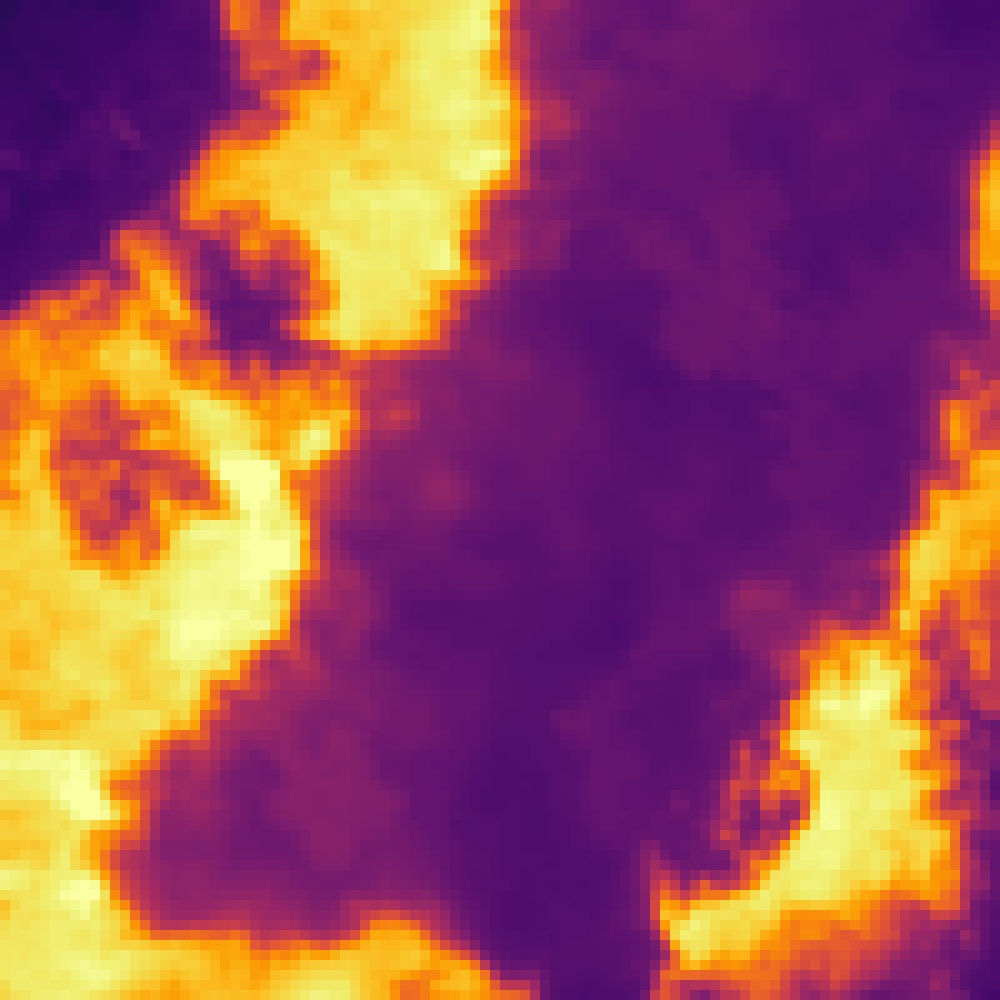
\includegraphics[width=0.75\linewidth]{img/experimentacion/naturales/Flame3/clean_04.jpg}
			\caption{Reducción por convolución}
			\label{fig:experimentacion:natuales:Flame3:clean_04}
		\end{subfigure}
		\hfill 
		\begin{subfigure}[b]{0.30\textwidth}
			\centering
			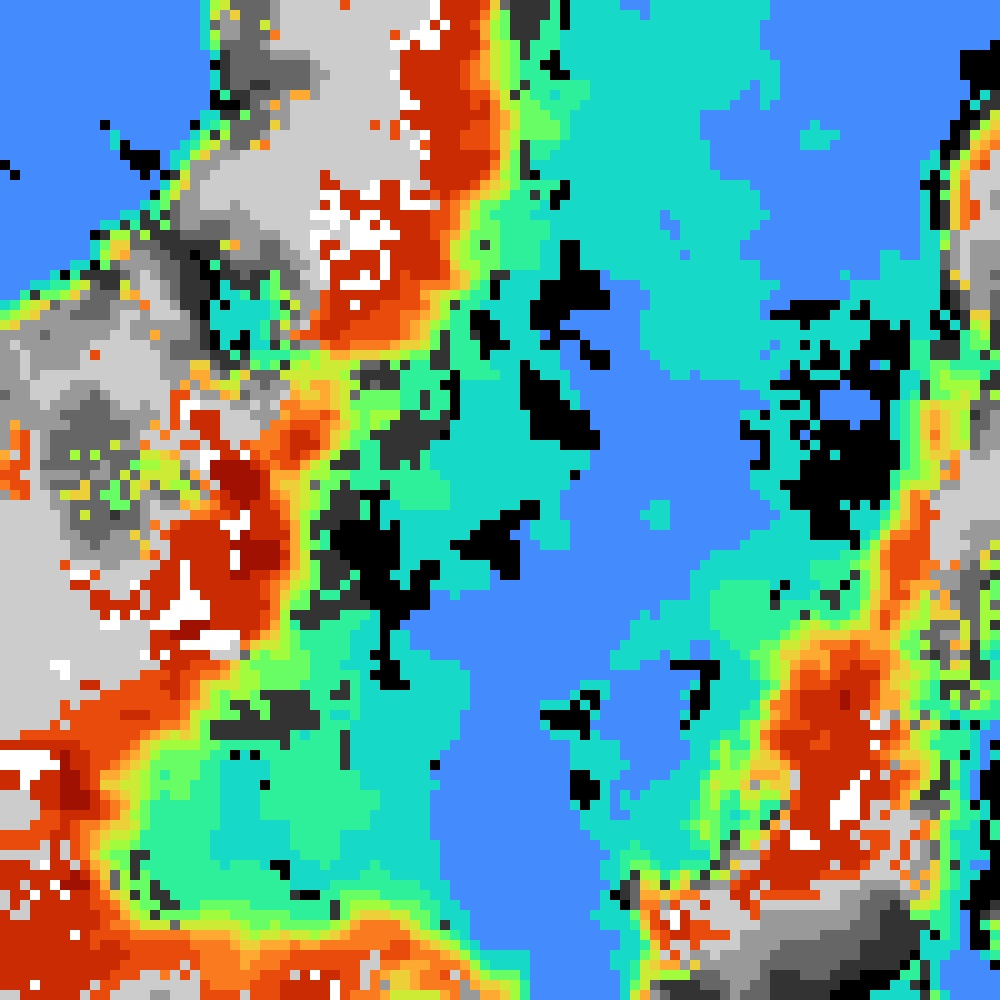
\includegraphics[width=0.75\linewidth]{img/experimentacion/naturales/Flame3/clean_05_18estados.jpg}
			\caption{Segmentación en 18 estados}
			\label{fig:experimentacion:natuales:Flame3:clean_05}
		\end{subfigure}
		\caption{Proceso de limpieza sobre la imagen 1204 del \textit{plot} 2 de Kaggle.}
		\label{fig:flame_clean_process}
	\end{figure}
	
		Con estos datos, obtenemos un total de $116 + 66 = 182$ imágenes de $100 \times 100$ píxeles, o mejor dicho, células. Estas tienen una distribución de estados como se muestra en la figura \ref{fig:flame_distribucion_estados}, en donde la mayoría de las células se ajustan a los valores más fríos, es decir, terreno que aún no se quema o que ya se enfrió después del fuego, y las zonas más calientes tienen menor representación. Sin embargo, se considera un rango aceptable dadas las capacidades de extracción de comportamientos que se apreciaron durante los experimentos de la hormiga de Langton.
	
	\begin{figure}[htbp]
		\centering
		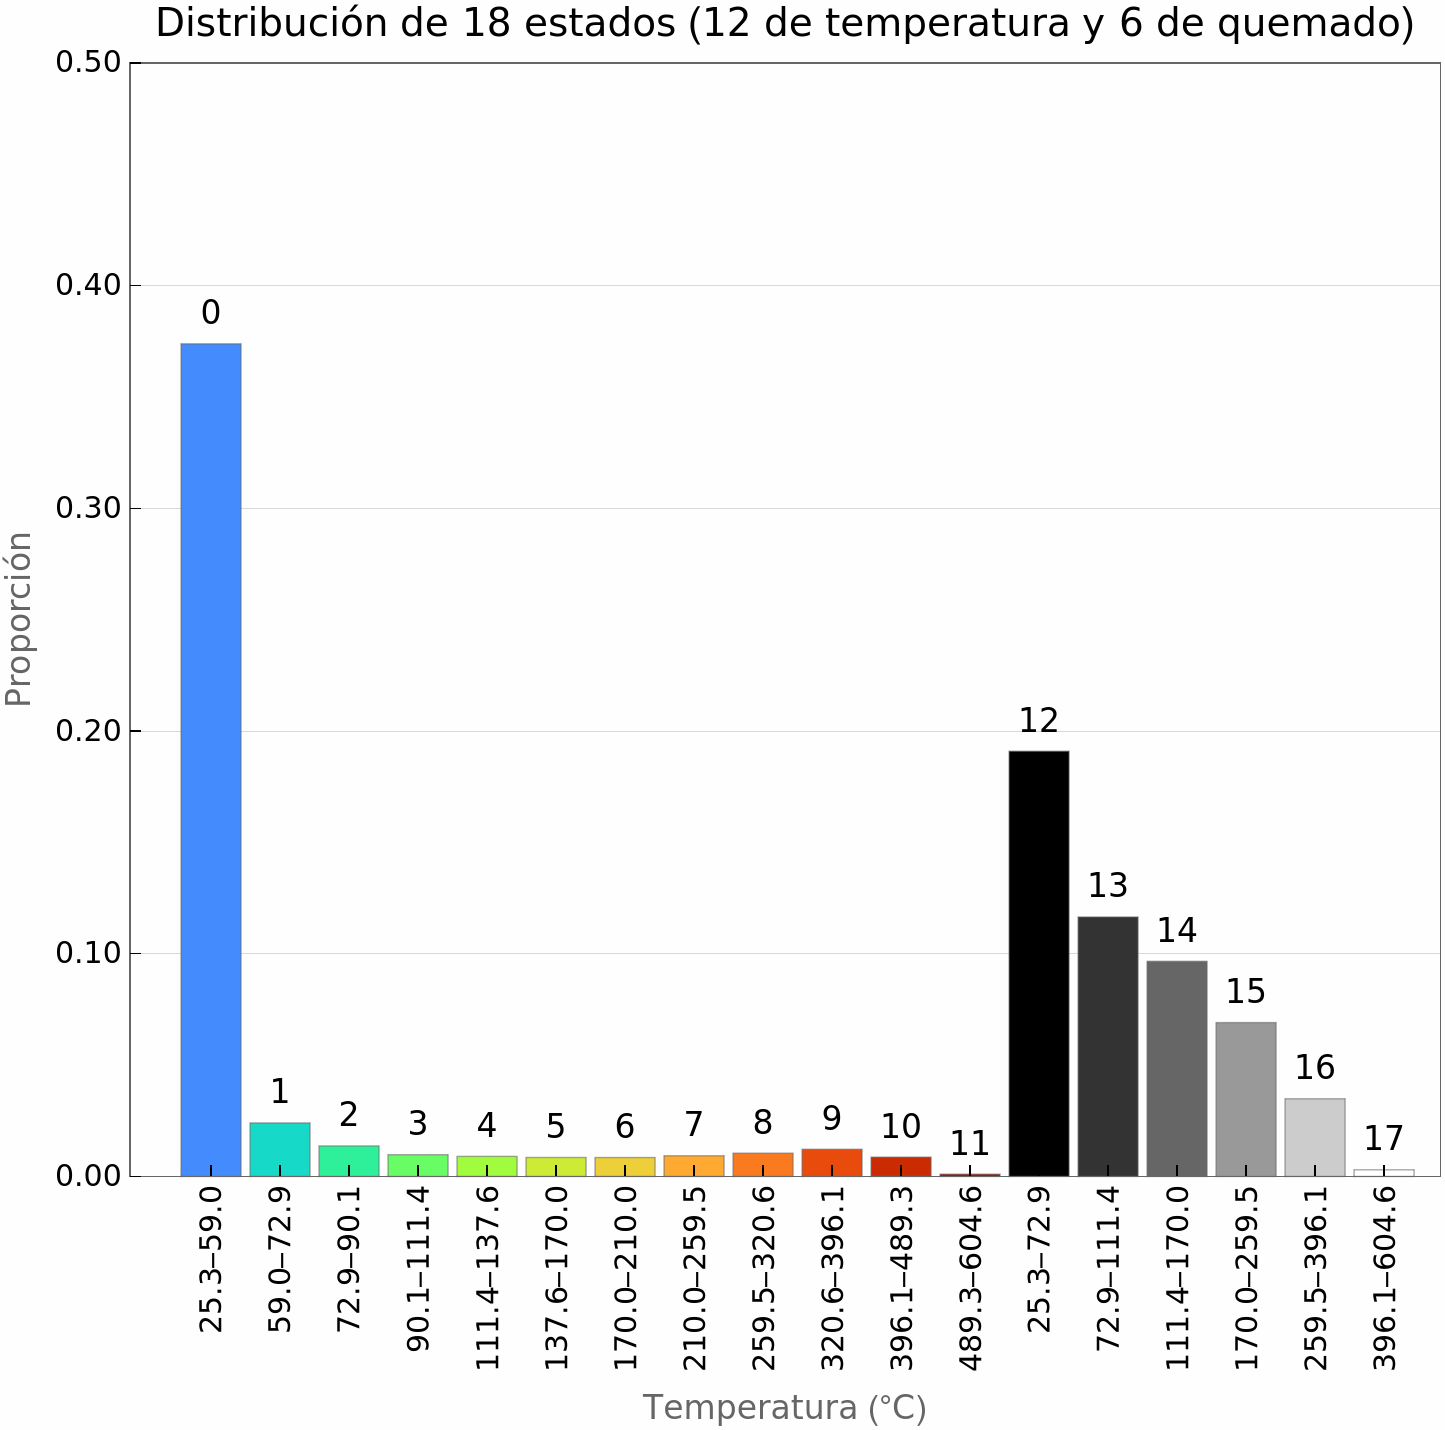
\includegraphics[width=0.6\linewidth]{img/experimentacion/naturales/Flame3/distribucion_estados18.png}
		\caption{Distribución de los 18 estados del conjunto de imágenes de entrenamiento de FLAME~3 para la predicción de propagación del fuego.}
		\label{fig:flame_distribucion_estados}
	\end{figure}
	
	Cabe mencionar que este método de limpieza de datos fue el que tuvo un mejor rendimiento y fue diseñado con base en los resultados de experimentos previos. 

	Adicionalmente, se hace la distinción entre el error de cuantización y el error de la dinámica: el primero mide qué tanta información se pierde al convertir una temperatura en un estado; no está relacionado con la red neuronal, únicamente mide la pérdida de información al discretizar. El segundo se refiere al error que tiene la red neuronal en su predicción, es decir, compara los datos discretizados con lo que predice la red.

	Por ejemplo, al discretizar en 15 estados con una escala logarítmica, tenemos un error de cuantización de 5.2 °C, es decir, en promedio cada célula difiere de su temperatura original por esa cantidad. A continuación, en la tabla \ref{tab:flame_experiments} se muestran múltiples configuraciones que ayudaron a obtener esta configuración final. El porcentaje de error en la predicción compara la red neuronal entrenada contra no hacer nada, es decir, contra suponer que cada célula conserva el mismo estado. Por esto, si es menor al 100\%, significa que la red mejora en relación con no hacer nada; en el caso contrario, es peor que no hacer nada.
	

	\begin{table}[htbp]
		\centering
		\footnotesize
		\setlength{\tabcolsep}{4pt}
		\setlength{\belowrulesep}{2pt}
		\begin{tabularx}{\textwidth}{p{0.24\textwidth}Xp{0.21\textwidth}}
			\toprule
			\textbf{Modificación} & \textbf{Resultado} & \textbf{Aporte a la configuración final} \\ \midrule
			Segmentar los estados mediante \textit{k-means} &
			Codo en $k = 4$. El estado 0 abarca del 66 al 99\% de las células y todo lo que supera 238 °C queda en un solo estado. &
			Escala logarítmica de 15 estados que distingue las zonas más calientes. \\ \midrule
			
			Tomar una imagen de cada 1, 3 o 6 &
			Con 6, la red de vecindad $9 \times 9$ y configuración 2:32 supera a la predicción sin cambio (exactitud de 0.588 contra 0.552 en el \textit{plot} de prueba). &
			Se toma una imagen de cada 6. \\ \midrule
			
			Cambiar el número de estados (de 4 a 50, logarítmicos y \textit{k-means}) &
			Con 50 estados se reduce el error de cuantización a 1.6 °C, pero no el error de la dinámica. Con 4 estados aumenta a 19 °C. &
			Entre 12 y 15 estados de temperatura (error de $\sim 5.2$ °C). \\ \midrule
			
			Quitar las imágenes de la ignición &
			Casi ninguna red supera a la predicción sin cambio ni enciende células. Las redes entrenadas con la ignición y evaluadas sin ella tienen menor error en la simulación libre. &
			Las secuencias inician con el fuego ya presente y en propagación. \\ \midrule
			
			Quitar el conjunto casi sin fuego &
			En ese conjunto casi nada cambia: la predicción sin cambio tiene un error de 1.92 °C y no permite saber si la red aprende. &
			Se descartan las secuencias casi sin fuego. \\ \midrule
			
			Unir los estados más fríos (0--2 en 13 estados; 0--3 en 12 estados) &
			Con 13, el error en la simulación libre baja de 21.9 a 19.2 °C. Con 12 estados, la mejor red tiene el 92.8\% del error de la predicción sin cambio. &
			12 estados de temperatura (estado 0 = 25.3--59.0 °C). \\ \midrule
			
			Rotar las imágenes de entrenamiento 0, 90, 180 y 270° &
			El error de un paso baja del 94 al 91\% del de la predicción sin cambio; la simulación libre no mejora de forma consistente. &
			No se usa. \\ \midrule
			Reducir a $200 \times 200$ &
			Error del 90\% de la predicción sin cambio, pero enciende menos células: solo el 50\% y el 20\% de las que se encienden tienen fuego vecino. &
			Se mantiene $100 \times 100$. \\ \midrule
			
			Agregar el combustible como clase fija &
			La red casi no enciende células (menos del 1.4\%) y no mejora a la red sin clase. &
			No se usa. \\ \midrule
			
			Bandera de quemado: el estado se duplica si la célula alguna vez llegó a 135.9 °C o más &
			5 veces más células encendidas, con precisión de $\approx 0.2$. Error de un paso de $\approx 22$ °C contra 16 °C de la predicción sin cambio, y la simulación libre diverge (37--67 °C contra 18 °C). &
			Estado de quemado por enfriamiento de la célula y no por un umbral fijo. \\ \midrule
			
			Quemado al enfriarse, con 12 estados de quemado (24 estados) y sin umbral &
			28,537 regresos de quemado a no quemado, el 92\% por subidas de un solo estado (ruido); el estado 23 nunca aparece. &
			Estados de quemado agrupados de dos en dos y umbral de 30 °C (9,102 regresos). \\ \bottomrule
			
		\end{tabularx}
		\caption{Modificaciones al preprocesamiento de FLAME~3 previas a la configuración final. Predicción sin cambio: suponer que el siguiente paso es igual al actual. Salvo que se indique otra cosa, vecindad $9 \times 9$, 2 capas de 32 neuronas e imágenes de $100 \times 100$.}
		\label{tab:flame_experiments}
	\end{table}
	
	Antes de definir estados de quemado o de combustible, usar \textit{one-hot encoding} no mejoraba los resultados (tabla \ref{tab:flame_onehot}). Con \textit{one-hot} la red aprende mejor los datos de entrenamiento, pero tiene una peor generalización: su error es mayor en casi todos los experimentos y entre 2 y 5 veces más redes terminan la simulación libre con más del doble de error que la predicción sin cambio. La excepción es la bandera de quemado, en donde los estados ya no están ordenados por temperatura.

	\begin{table}[htbp]
		\centering
		\footnotesize
		\setlength{\tabcolsep}{4pt}
		\begin{tabular}{llcccc}
			\toprule
			& & \textbf{Error} & \textbf{Redes} & & \\
			& & \textbf{respecto a} & \textbf{mejores que} & & \\
			& & \textbf{la predicción} & \textbf{la predicción} & \textbf{Redes que} & \textbf{Pérdida al} \\
			\textbf{Experimento} & \textbf{One-hot} & \textbf{sin cambio} & \textbf{sin cambio} & \textbf{se desvían} & \textbf{entrenar} \\ \midrule
			\multirow{2}{*}{Paso de 1 imagen} & No & 104\% & 0 de 18 & 1 de 18 & 0.225 \\
			& Sí & 111\% & 0 de 18 & 4 de 18 & 0.208 \\ \midrule
			\multirow{2}{*}{Pasos de 3 y 6} & No & 109\% & 6 de 24 & 5 de 24 & 0.417 \\
			& Sí & 121\% & 4 de 24 & 11 de 24 & 0.352 \\ \midrule
			\multirow{2}{*}{Sin ignición} & No & 113\% & 11 de 36 & 3 de 36 & 0.447 \\
			& Sí & 132\% & 7 de 36 & 15 de 36 & 0.371 \\ \midrule
			\multirow{2}{*}{Rotaciones} & No & 101\% & 23 de 48 & 4 de 48 & 0.613 \\
			& Sí & 105\% & 15 de 48 & 16 de 48 & 0.523 \\ \midrule
			\multirow{2}{*}{4 estados} & No & 103\% & 7 de 20 & 0 de 20 & 0.255 \\
			& Sí & 103\% & 6 de 20 & 6 de 20 & 0.215 \\ \midrule
			\multirow{2}{*}{Bandera de quemado} & No & 111\% & 9 de 16 & 2 de 16 & 0.645 \\
			& Sí & 100\% & 11 de 16 & 4 de 16 & 0.523 \\ \bottomrule
		\end{tabular}
		\caption{Las mismas redes entrenadas sin y con \textit{one-hot encoding}. Redes que se desvían: redes que al final de la simulación libre tienen más del doble del error de la predicción sin cambio.}
		\label{tab:flame_onehot}
	\end{table}

	\subsection{Capacidad de replicación}

	Con los 18 estados (12 de temperatura y 6 de quemado) se probaron 18 configuraciones: paso de 5, 15 o 30 s (1 \textit{frame} = 5 s); vecindad de $9 \times 9$ (81 vecinos) o dispersa (41 vecinos), y capas ocultas de 2:32:ReLU, 3:64:ReLU o 4:256:ReLU, con capa de salida 18:Linear. Todas usan \textit{one-hot}, por lo que la capa de entrada tiene $81 \times 18 = 1{,}458$ entradas con la vecindad de $9 \times 9$ y $41 \times 18 = 738$ con la dispersa. Cada configuración se entrenó con un conjunto y se probó en el otro: primero se entrena con flame\_plot\_2 y se prueba en flame\_plot\_1, y después al revés. En la prueba, la red parte de la primera imagen y evoluciona sola con sus propias predicciones (simulación libre) hasta el final de la secuencia.

	La vecindad dispersa toma el cuadrado de $5 \times 5$ alrededor de la célula y 16 células a distancia 5: las cuatro esquinas y tres células en el centro de cada lado de un cuadrado de $11 \times 11$ (figura \ref{fig:flame_vecindades}). Solo se usan vecindades de 128 vecinos o menos, que es el máximo que acepta el simulador; por ejemplo, una vecindad de $13 \times 13$ tiene 169 vecinos.

	\begin{figure}[htbp]
		\centering
		\begin{subfigure}[b]{0.30\textwidth}
			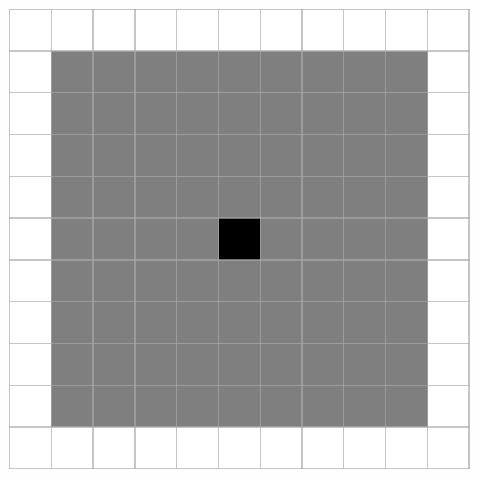
\includegraphics[width=\textwidth]{img/experimentacion/naturales/Flame3/vecindad_9x9.png}
			\caption{Vecindad de $9 \times 9$ (81 vecinos).}
			\label{fig:flame_vecindad_9x9}
		\end{subfigure}
		\hspace{1cm}
		\begin{subfigure}[b]{0.30\textwidth}
			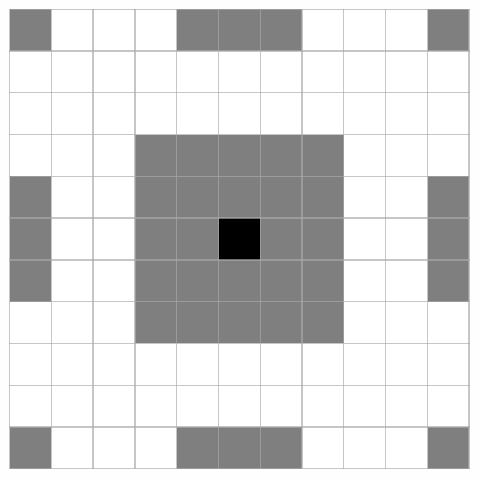
\includegraphics[width=\textwidth]{img/experimentacion/naturales/Flame3/vecindad_dispersa41.png}
			\caption{Vecindad dispersa (41 vecinos).}
			\label{fig:flame_vecindad_dispersa}
		\end{subfigure}
		\caption{Vecindades de las 18 configuraciones. La célula central, en negro, también es parte de la vecindad.}
		\label{fig:flame_vecindades}
	\end{figure}

	Todas las configuraciones se entrenaron durante 200 épocas con entropía cruzada como función de pérdida, una tasa de aprendizaje inicial de 0.001 con reducción exponencial hasta 0.00001, un tamaño del lote de 8,192, frontera abierta y semilla aleatoria 42. Para aprovechar todas las imágenes, con un paso de 30 s cada conjunto se divide en 6 secuencias que empiezan en imágenes distintas (0, 6, 12, \dots; 1, 7, 13, \dots; y así hasta 5, 11, 17, \dots) y las 6 se usan para entrenar; con un paso de 15 s se forman 3 secuencias y con uno de 5 s, solo una.

	Para comparar las configuraciones se usan cuatro medidas. Para el área quemada y el área con fuego, un valor de 100\% significa que la simulación libre es idéntica a la real. Para los dos errores, un valor de 100\% significa que la red se equivocó en la misma medida que la predicción sin cambio; menos de 100\% significa que la red es mejor y más de 100\%, que es peor. Por ejemplo, un error de 89\% indica que la red se equivoca 11\% menos que la predicción sin cambio, mientras que uno de 400\% indica que se equivoca cuatro veces más. 
	
	\begin{enumerate}
		\item El área quemada indica qué tanto se parece el área quemada al final de la simulación libre a la real.
		\item El área con fuego indica qué tanto se parecen las células que alguna vez llegaron a 130 °C.
		\item El error de un paso se mide prediciendo un solo paso desde cada imagen real.
		\item El error en la simulación libre se mide en su último paso.
	\end{enumerate} 

	Como de un paso a otro el fuego cambia pocas células, la predicción sin cambio tiene un error bajo y es difícil de superar; sin embargo, nunca propaga el fuego, por lo que su área quemada es de 0\%. Por esto, el área quemada indica si la red propaga el fuego hacia donde debe, y el error, si además acierta las temperaturas.

	Las configuraciones también se evaluaron de forma visual, eligiendo las mejores al ver la animación de la simulación libre junto a la evolución real (columna ``Selección visual''). Esta selección coincide con el área quemada: al probar en flame\_plot\_1 se eligieron las 5 primeras por área quemada, y al probar en flame\_plot\_2, la primera y la tercera. Esto indica que el área quemada es la medida que mejor representa si la simulación se parece a la propagación real. Las configuraciones elegidas de forma visual cumplen los siguientes criterios:
	
	\begin{itemize}
		\item Propagan el fuego a una velocidad constante y similar a la de la evolución de prueba.
		\item Si se inicia el sistema con una frontera periódica y con el fuego en el centro, los frentes de propagación del fuego se extinguen al colisionar.
		\item Una vez quemado todo el sistema, este ya no es capaz de generar fuego.
		\item El sistema se calienta y se enfría.
	\end{itemize}

	La tabla \ref{tab:flame_18_prueba1} muestra los resultados al probar en flame\_plot\_1. A diferencia de los experimentos sin estados de quemado, todas las configuraciones propagan el fuego: el área quemada se parece entre un 72 y un 86\% a la real. Las mejores son las redes de 2:32 y 3:64 con paso de 15 y 30 s, con un área quemada del 84 al 86\%. Sin embargo, ninguna supera a la predicción sin cambio en el error de la simulación libre: las de paso de 30 s se equivocan entre 1.4 y 2.3 veces más, y las de paso de 15 s, entre 3.6 y 4.5 veces más. Es decir, el fuego avanza hacia las zonas correctas, pero las temperaturas no coinciden con las reales.

	\begin{table}[htbp]
		\centering
		\footnotesize
		\setlength{\tabcolsep}{3pt}
		\begin{tabular}{@{}ccccccccc@{}}
			\toprule
			& & & & & & \textbf{Error en la} & & \\
			& & & & \textbf{Área} & \textbf{Área} & \textbf{simulación} & \textbf{Error de} & \textbf{Selección} \\
			\textbf{Lugar} & \textbf{Paso} & \textbf{Vecindad} & \textbf{Capas} & \textbf{quemada} & \textbf{con fuego} & \textbf{libre} & \textbf{un paso} & \textbf{visual} \\ \midrule
			1 & 15 s & Dispersa & 3:64 & 86\% & 68\% & 404\% & 113\% & $\checkmark$ \\
			2 & 30 s & Dispersa & 3:64 & 86\% & 67\% & 140\% & 119\% & $\checkmark$ \\
			3 & 30 s & $9 \times 9$ & 2:32 & 85\% & 55\% & 147\% & 110\% & $\checkmark$ \\
			4 & 15 s & $9 \times 9$ & 2:32 & 85\% & 57\% & 450\% & 108\% & $\checkmark$ \\
			5 & 15 s & $9 \times 9$ & 3:64 & 85\% & 68\% & 391\% & 118\% & $\checkmark$ \\
			6 & 30 s & Dispersa & 2:32 & 84\% & 67\% & 232\% & 114\% &  \\
			7 & 15 s & Dispersa & 2:32 & 84\% & 38\% & 364\% & 106\% &  \\
			8 & 30 s & $9 \times 9$ & 3:64 & 84\% & 65\% & 170\% & 125\% & $\checkmark$ \\
			9 & 5 s & Dispersa & 4:256 & 83\% & 69\% & 709\% & 119\% &  \\
			10 & 5 s & $9 \times 9$ & 4:256 & 79\% & 69\% & 429\% & 126\% &  \\
			11 & 15 s & $9 \times 9$ & 4:256 & 79\% & 68\% & 326\% & 145\% &  \\
			12 & 15 s & Dispersa & 4:256 & 78\% & 68\% & 287\% & 140\% & $\checkmark$ \\
			% 13 & 5 s & $9 \times 9$ & 2:32 & 74\% & 71\% & 1203\% & 102\% &  \\
			% 14 & 30 s & Dispersa & 4:256 & 74\% & 67\% & 382\% & 145\% &  \\
			% 15 & 5 s & Dispersa & 3:64 & 74\% & 69\% & 1179\% & 102\% &  \\
			% 16 & 30 s & $9 \times 9$ & 4:256 & 73\% & 66\% & 471\% & 148\% &  \\
			% 17 & 5 s & $9 \times 9$ & 3:64 & 73\% & 69\% & 909\% & 107\% &  \\
			% 18 & 5 s & Dispersa & 2:32 & 72\% & 70\% & 1195\% & 101\% &  \\
			\bottomrule
		\end{tabular}
		\caption{Las 12 mejores configuraciones probadas en flame\_plot\_1 y entrenadas con flame\_plot\_2, ordenadas por área quemada.}
		\label{tab:flame_18_prueba1}
	\end{table}

	

	La tabla \ref{tab:flame_18_prueba2} muestra los resultados al probar en flame\_plot\_2, en donde el fuego es más difícil de reproducir: el área quemada se parece como máximo en un 67\% a la real. En este caso las mejores son las redes de 4:256, ya que las redes de 2:32 propagan el fuego muy lento y su área quemada se queda entre el 10 y el 30\%. En esta prueba varias configuraciones sí superan a la predicción sin cambio en la simulación libre, como la de $9 \times 9$ con 4:256 y paso de 15 s, que tiene el área quemada más parecida (67\%) y se equivoca un 11\% menos que la predicción sin cambio.


	\begin{table}[htbp]
		\centering
		\footnotesize
		\setlength{\tabcolsep}{3pt}
		\begin{tabular}{@{}ccccccccc@{}}
			\toprule
			& & & & & & \textbf{Error en la} & & \\
			& & & & \textbf{Área} & \textbf{Área} & \textbf{simulación} & \textbf{Error de} & \textbf{Selección} \\
			\textbf{Lugar} & \textbf{Paso} & \textbf{Vecindad} & \textbf{Capas} & \textbf{quemada} & \textbf{con fuego} & \textbf{libre} & \textbf{un paso} & \textbf{visual} \\ \midrule
			1 & 15 s & $9 \times 9$ & 4:256 & 67\% & 61\% & 89\% & 105\% & $\checkmark$ \\
			2 & 5 s & Dispersa & 4:256 & 61\% & 52\% & 77\% & 117\% &  \\
			3 & 5 s & $9 \times 9$ & 4:256 & 57\% & 44\% & 87\% & 118\% & $\checkmark$ \\
			4 & 15 s & Dispersa & 4:256 & 50\% & 44\% & 94\% & 104\% &  \\
			5 & 30 s & $9 \times 9$ & 4:256 & 49\% & 44\% & 96\% & 93\% &  \\
			6 & 15 s & $9 \times 9$ & 3:64 & 43\% & 41\% & 99\% & 104\% &  \\
			7 & 15 s & Dispersa & 3:64 & 40\% & 40\% & 112\% & 100\% &  \\
			8 & 30 s & Dispersa & 4:256 & 39\% & 34\% & 94\% & 92\% &  \\
			9 & 30 s & $9 \times 9$ & 3:64 & 36\% & 33\% & 102\% & 93\% &  \\
			10 & 30 s & Dispersa & 3:64 & 33\% & 29\% & 101\% & 90\% &  \\
			11 & 30 s & $9 \times 9$ & 2:32 & 30\% & 27\% & 97\% & 89\% &  \\
			12 & 5 s & $9 \times 9$ & 3:64 & 28\% & 27\% & 126\% & 110\% &  \\
			% 13 & 30 s & Dispersa & 2:32 & 25\% & 20\% & 97\% & 88\% &  \\
			% 14 & 15 s & $9 \times 9$ & 2:32 & 23\% & 19\% & 98\% & 101\% &  \\
			% 15 & 15 s & Dispersa & 2:32 & 22\% & 21\% & 107\% & 101\% &  \\
			% 16 & 5 s & Dispersa & 3:64 & 21\% & 21\% & 129\% & 106\% &  \\
			% 17 & 5 s & $9 \times 9$ & 2:32 & 16\% & 23\% & 149\% & 108\% &  \\
			% 18 & 5 s & Dispersa & 2:32 & 10\% & 28\% & 173\% & 104\% &  \\
			\bottomrule
		\end{tabular}
		\caption{Las 12 mejores configuraciones probadas en flame\_plot\_2 y entrenadas con flame\_plot\_1, ordenadas por área quemada.}
		\label{tab:flame_18_prueba2}
	\end{table}

	
	Ninguna configuración es la mejor en las dos pruebas: las redes chicas funcionan mejor en flame\_plot\_1 y las grandes en flame\_plot\_2. Para elegir una configuración general, en la tabla \ref{tab:flame_18_lugares} se ordenan las configuraciones de la 1 (mejor) a la 18 en cada prueba y se promedia su lugar. Considerando solo el área quemada, las mejores son la dispersa con 3:64 y paso de 15 s, la de $9 \times 9$ con 3:64 y paso de 15 s, y la dispersa con 4:256 y paso de 5 s. Considerando las cuatro medidas (lugar combinado), las mejores son la dispersa con 3:64 y paso de 15 o 30 s, y la de $9 \times 9$ con 2:32 y paso de 30 s. En ambos casos, las peores son las de paso de 5 s con redes de 2:32 o 3:64: las células quemadas no se enfrían y el error en la simulación libre llega a ser 12 veces el de la predicción sin cambio.

	\begin{table}[htbp]
		\centering
		\footnotesize
		\setlength{\tabcolsep}{3pt}
		\begin{tabular}{ccccccccc}
			\toprule
			& & & \multicolumn{3}{c}{\textbf{Lugar por área quemada}} & \multicolumn{3}{c}{\textbf{Lugar combinado}} \\
			\cmidrule(lr){4-6} \cmidrule(lr){7-9}
			& & & \textbf{Prueba} & \textbf{Prueba} & & \textbf{Prueba} & \textbf{Prueba} & \\
			\textbf{Paso} & \textbf{Vecindad} & \textbf{Capas} & \textbf{1} & \textbf{2} & \textbf{Promedio} & \textbf{1} & \textbf{2} & \textbf{Promedio} \\ \midrule
			15 s & Dispersa & 3:64 & 1 & 7 & 4 & 1 & 10 & 5.5 \\
			15 s & $9 \times 9$ & 3:64 & 5 & 6 & 5.5 & 5 & 7 & 6 \\
			5 s & Dispersa & 4:256 & 9 & 2 & 5.5 & 9.5 & 3 & 6.25 \\
			30 s & Dispersa & 3:64 & 2 & 10 & 6 & 2 & 9 & 5.5 \\
			15 s & $9 \times 9$ & 4:256 & 11 & 1 & 6 & 14 & 1 & 7.5 \\
			5 s & $9 \times 9$ & 4:256 & 10 & 3 & 6.5 & 9.5 & 6 & 7.75 \\
			30 s & $9 \times 9$ & 2:32 & 3 & 11 & 7 & 3 & 8 & 5.5 \\
			15 s & Dispersa & 4:256 & 12 & 4 & 8 & 15.5 & 4.5 & 10 \\
			30 s & $9 \times 9$ & 3:64 & 8 & 9 & 8.5 & 12 & 11 & 11.5 \\
			15 s & $9 \times 9$ & 2:32 & 4 & 14 & 9 & 9.5 & 13 & 11.25 \\
			30 s & Dispersa & 2:32 & 6 & 13 & 9.5 & 4 & 12 & 8 \\
			30 s & $9 \times 9$ & 4:256 & 16 & 5 & 10.5 & 18 & 2 & 10 \\
			15 s & Dispersa & 2:32 & 7 & 15 & 11 & 7 & 14 & 10.5 \\
			30 s & Dispersa & 4:256 & 14 & 8 & 11 & 17 & 4.5 & 10.75 \\
			5 s & $9 \times 9$ & 3:64 & 17 & 12 & 14.5 & 15.5 & 15 & 15.25 \\
			5 s & $9 \times 9$ & 2:32 & 13 & 17 & 15 & 6 & 18 & 12 \\
			5 s & Dispersa & 3:64 & 15 & 16 & 15.5 & 13 & 17 & 15 \\
			5 s & Dispersa & 2:32 & 18 & 18 & 18 & 9.5 & 16 & 12.75 \\ \bottomrule
		\end{tabular}
		\caption{Lugar de cada configuración (1 = mejor) entre las 18, ordenadas por el promedio del lugar por área quemada.}
		\label{tab:flame_18_lugares}
	\end{table}

	Las tres configuraciones con mejor lugar combinado empatan con 5.5. De ellas, se elige como configuración final la de paso de 30 s, vecindad de $9 \times 9$ y 2:32:ReLU, por ser la red más pequeña y la única de las tres que, al probar en flame\_plot\_2, se equivoca menos que la predicción sin cambio tanto en un paso (89\%) como en la simulación libre (97\%).

	La figura \ref{fig:flame_criterios} muestra la configuración final en el simulador con los criterios de la selección visual. El espacio inicia frío y sin quemar, con un foco de fuego en el centro y frontera periódica: el fuego se propaga en todas direcciones (b y c), los frentes se extinguen al encontrarse después de cruzar la frontera (d y e) y, una vez quemado todo el espacio, ya no vuelve a aparecer fuego (f).

	% Leyenda de los 18 estados con la paleta del simulador (Simulator/GUI/colores/flame_log12_quemado6.csv)
	\definecolor{flame0}{HTML}{448CFD}\definecolor{flame1}{HTML}{17D9C7}\definecolor{flame2}{HTML}{2FF09A}
	\definecolor{flame3}{HTML}{69FD65}\definecolor{flame4}{HTML}{A1FC3D}\definecolor{flame5}{HTML}{CDEB34}
	\definecolor{flame6}{HTML}{EDCF39}\definecolor{flame7}{HTML}{FDA932}\definecolor{flame8}{HTML}{FA7A1F}
	\definecolor{flame9}{HTML}{E84B0C}\definecolor{flame10}{HTML}{CB2B03}\definecolor{flame11}{HTML}{A01101}
	\definecolor{flame12}{HTML}{000000}\definecolor{flame13}{HTML}{333333}\definecolor{flame14}{HTML}{666666}
	\definecolor{flame15}{HTML}{999999}\definecolor{flame16}{HTML}{CCCCCC}\definecolor{flame17}{HTML}{FFFFFF}
	\newcommand{\estadoflame}[2][black]{\fcolorbox{gray}{flame#2}{\makebox[1.1em]{\textcolor{#1}{#2}}}}
	\newcommand{\leyendaflame}{%
		\par\medskip
		{\footnotesize\setlength{\fboxsep}{1pt}%
		Temperatura: \estadoflame{0}\estadoflame{1}\estadoflame{2}\estadoflame{3}\estadoflame{4}\estadoflame{5}%
		\estadoflame{6}\estadoflame{7}\estadoflame{8}\estadoflame{9}\estadoflame[white]{10}\estadoflame[white]{11}%
		\quad Quemado: \estadoflame[white]{12}\estadoflame[white]{13}\estadoflame[white]{14}\estadoflame{15}%
		\estadoflame{16}\estadoflame{17}\par}}

	\begin{figure}[htbp]
		\centering
		\begin{subfigure}[t]{0.3\textwidth}
			\centering
			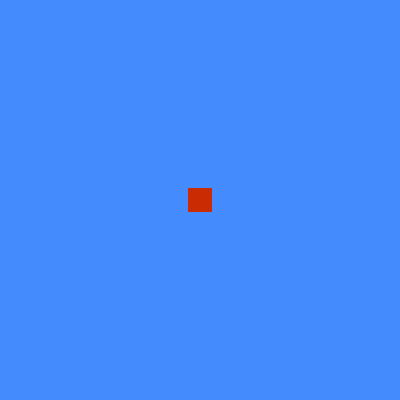
\includegraphics[width=\linewidth]{img/experimentacion/naturales/Flame3/criterios/entrenada_flame_plot_2/paso_0.png}
			\caption{0 s}
			\label{fig:flame_criterios_0s}
		\end{subfigure}
		\hfill
		\begin{subfigure}[t]{0.3\textwidth}
			\centering
			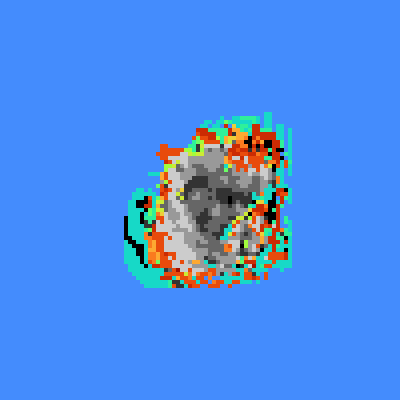
\includegraphics[width=\linewidth]{img/experimentacion/naturales/Flame3/criterios/entrenada_flame_plot_2/paso_5.png}
			\caption{150 s}
			\label{fig:flame_criterios_150s}
		\end{subfigure}
		\hfill
		\begin{subfigure}[t]{0.3\textwidth}
			\centering
			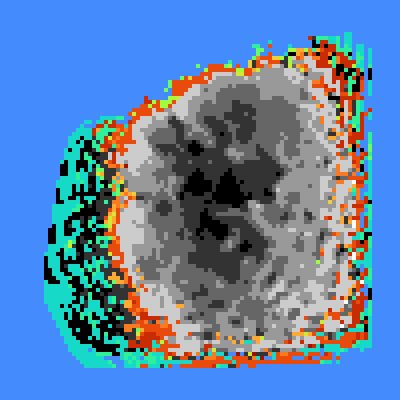
\includegraphics[width=\linewidth]{img/experimentacion/naturales/Flame3/criterios/entrenada_flame_plot_2/paso_10.png}
			\caption{300 s}
			\label{fig:flame_criterios_300s}
		\end{subfigure}
		\\[6pt]
		\begin{subfigure}[t]{0.3\textwidth}
			\centering
			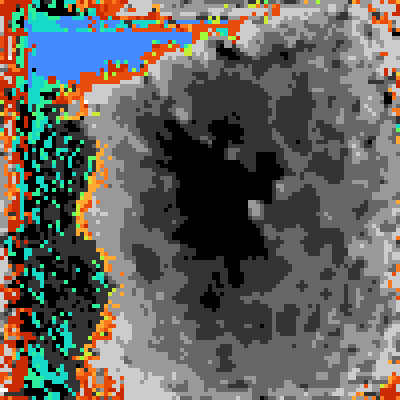
\includegraphics[width=\linewidth]{img/experimentacion/naturales/Flame3/criterios/entrenada_flame_plot_2/paso_14.png}
			\caption{420 s}
			\label{fig:flame_criterios_420s}
		\end{subfigure}
		\hfill
		\begin{subfigure}[t]{0.3\textwidth}
			\centering
			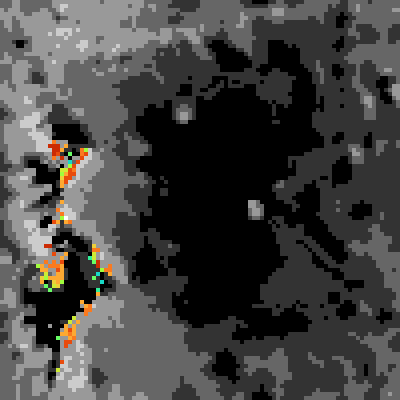
\includegraphics[width=\linewidth]{img/experimentacion/naturales/Flame3/criterios/entrenada_flame_plot_2/paso_18.png}
			\caption{540 s}
			\label{fig:flame_criterios_540s}
		\end{subfigure}
		\hfill
		\begin{subfigure}[t]{0.3\textwidth}
			\centering
			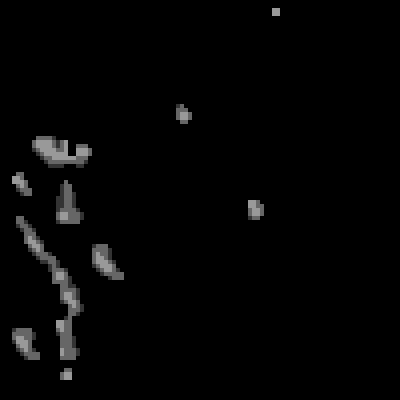
\includegraphics[width=\linewidth]{img/experimentacion/naturales/Flame3/criterios/entrenada_flame_plot_2/paso_40.png}
			\caption{1200 s}
			\label{fig:flame_criterios_1200s}
		\end{subfigure}
		\leyendaflame
		\caption{Configuración final (paso de 30 s, vecindad de $9 \times 9$ y 2:32:ReLU, entrenada con flame\_plot\_2) en el simulador, con frontera periódica. El espacio de $100 \times 100$ células inicia en el estado 0 con un foco de $6 \times 6$ células en el estado 10 en el centro. Los colores son los estados de la tabla \ref{tab:flame_states_proportion}.}
		\label{fig:flame_criterios}
	\end{figure}

	En las figuras \ref{fig:flame_comparacion1} y \ref{fig:flame_comparacion2} se muestran la evolución original y la comparativa con las 9 configuraciones de la selección visual de ambas pruebas, al probar en flame\_plot\_1 y en flame\_plot\_2, respectivamente.

	\begin{figure}[htbp]
		\centering
		\begin{subfigure}[t]{0.48\textwidth}
			\centering
			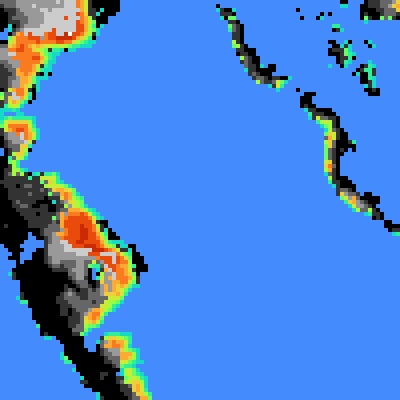
\includegraphics[width=0.32\linewidth]{img/experimentacion/naturales/Flame3/comparacion/flame_plot_1/real_150s.png}\hfill
			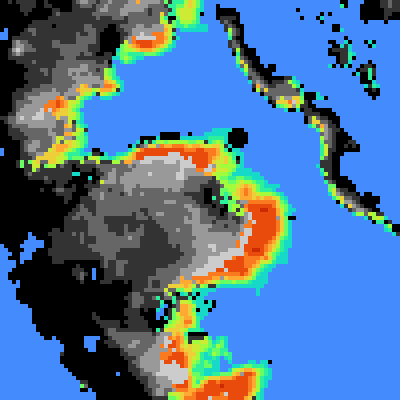
\includegraphics[width=0.32\linewidth]{img/experimentacion/naturales/Flame3/comparacion/flame_plot_1/real_300s.png}\hfill
			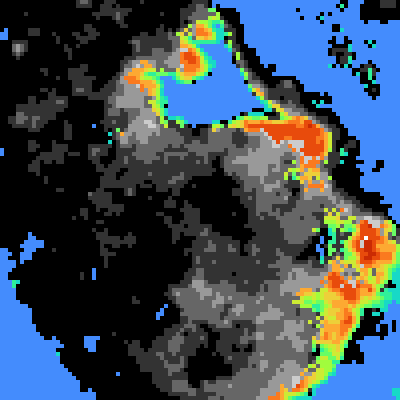
\includegraphics[width=0.32\linewidth]{img/experimentacion/naturales/Flame3/comparacion/flame_plot_1/real_420s.png}
			\caption{Real}
			\label{fig:flame_comparacion1_real}
		\end{subfigure}
		\hfill
		\begin{subfigure}[t]{0.48\textwidth}
			\centering
			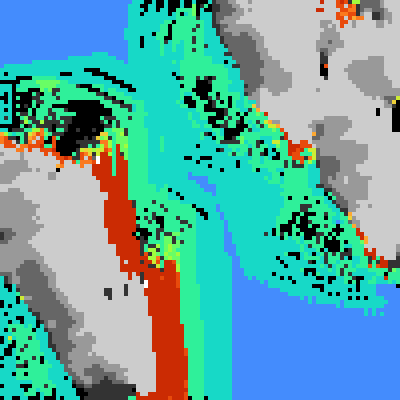
\includegraphics[width=0.32\linewidth]{img/experimentacion/naturales/Flame3/comparacion/flame_plot_1/paso15s_9x9_2x32_150s.png}\hfill
			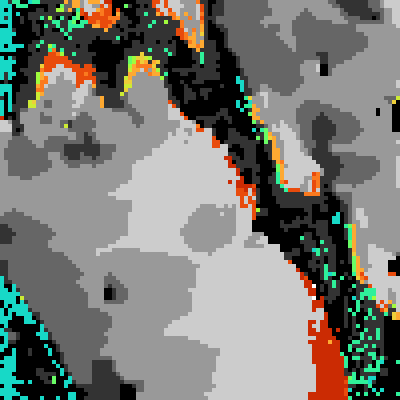
\includegraphics[width=0.32\linewidth]{img/experimentacion/naturales/Flame3/comparacion/flame_plot_1/paso15s_9x9_2x32_300s.png}\hfill
			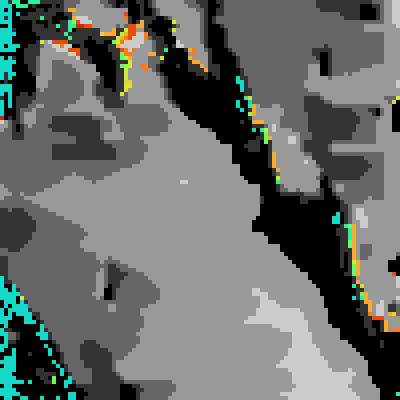
\includegraphics[width=0.32\linewidth]{img/experimentacion/naturales/Flame3/comparacion/flame_plot_1/paso15s_9x9_2x32_420s.png}
			\caption{15 s, $9 \times 9$, 2:32}
			\label{fig:flame_comparacion1_paso15s_9x9_2x32}
		\end{subfigure}
		\\[6pt]
		\begin{subfigure}[t]{0.48\textwidth}
			\centering
			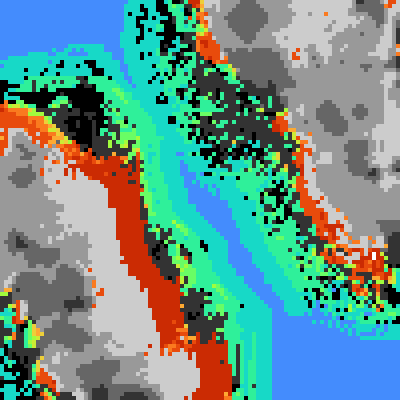
\includegraphics[width=0.32\linewidth]{img/experimentacion/naturales/Flame3/comparacion/flame_plot_1/paso15s_9x9_3x64_150s.png}\hfill
			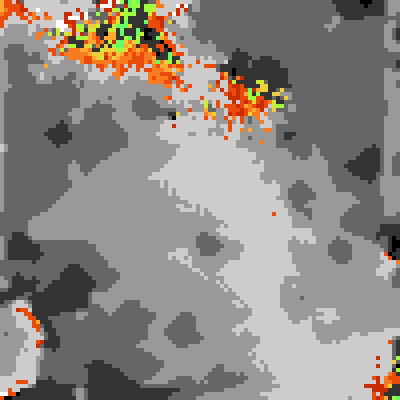
\includegraphics[width=0.32\linewidth]{img/experimentacion/naturales/Flame3/comparacion/flame_plot_1/paso15s_9x9_3x64_300s.png}\hfill
			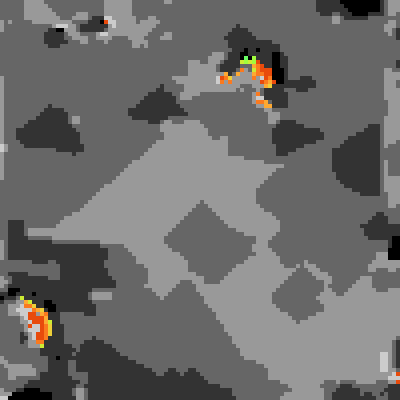
\includegraphics[width=0.32\linewidth]{img/experimentacion/naturales/Flame3/comparacion/flame_plot_1/paso15s_9x9_3x64_420s.png}
			\caption{15 s, $9 \times 9$, 3:64}
			\label{fig:flame_comparacion1_paso15s_9x9_3x64}
		\end{subfigure}
		\hfill
		\begin{subfigure}[t]{0.48\textwidth}
			\centering
			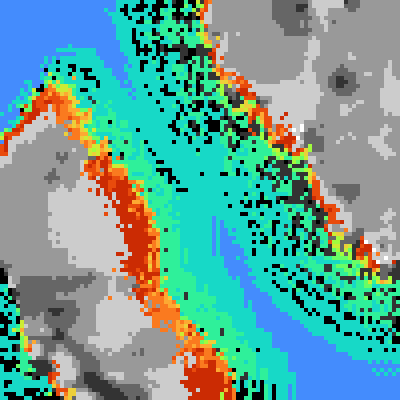
\includegraphics[width=0.32\linewidth]{img/experimentacion/naturales/Flame3/comparacion/flame_plot_1/paso15s_dispersa41_3x64_150s.png}\hfill
			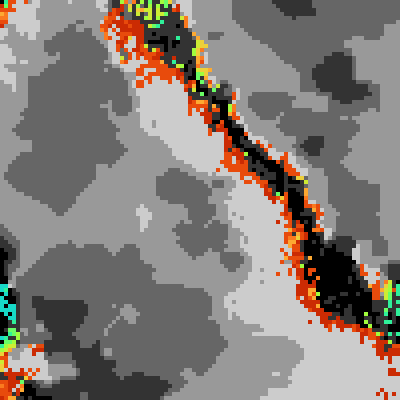
\includegraphics[width=0.32\linewidth]{img/experimentacion/naturales/Flame3/comparacion/flame_plot_1/paso15s_dispersa41_3x64_300s.png}\hfill
			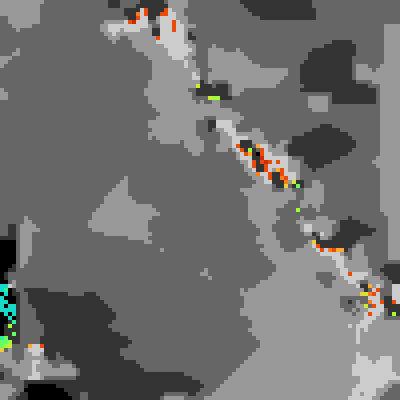
\includegraphics[width=0.32\linewidth]{img/experimentacion/naturales/Flame3/comparacion/flame_plot_1/paso15s_dispersa41_3x64_420s.png}
			\caption{15 s, dispersa, 3:64}
			\label{fig:flame_comparacion1_paso15s_dispersa41_3x64}
		\end{subfigure}
		\\[6pt]
		\begin{subfigure}[t]{0.48\textwidth}
			\centering
			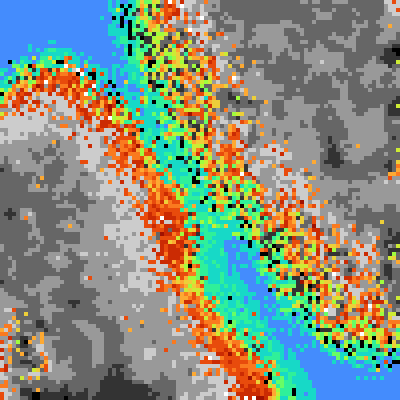
\includegraphics[width=0.32\linewidth]{img/experimentacion/naturales/Flame3/comparacion/flame_plot_1/paso15s_dispersa41_4x256_150s.png}\hfill
			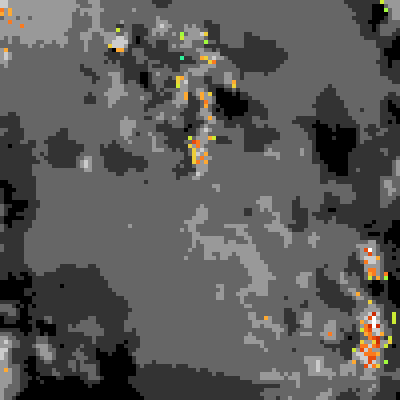
\includegraphics[width=0.32\linewidth]{img/experimentacion/naturales/Flame3/comparacion/flame_plot_1/paso15s_dispersa41_4x256_300s.png}\hfill
			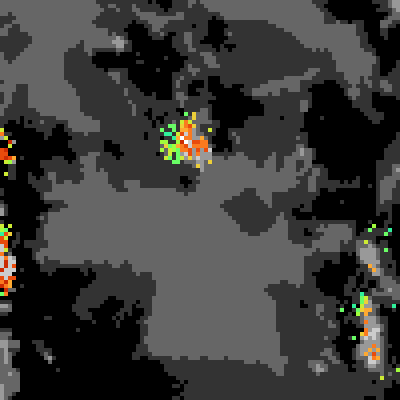
\includegraphics[width=0.32\linewidth]{img/experimentacion/naturales/Flame3/comparacion/flame_plot_1/paso15s_dispersa41_4x256_420s.png}
			\caption{15 s, dispersa, 4:256}
			\label{fig:flame_comparacion1_paso15s_dispersa41_4x256}
		\end{subfigure}
		\hfill
		\begin{subfigure}[t]{0.48\textwidth}
			\centering
			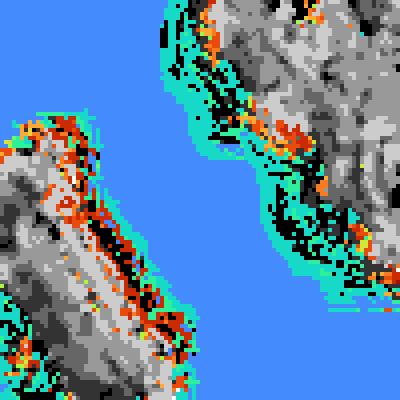
\includegraphics[width=0.32\linewidth]{img/experimentacion/naturales/Flame3/comparacion/flame_plot_1/paso30s_9x9_2x32_150s.png}\hfill
			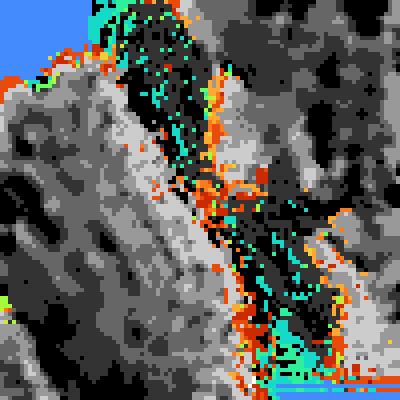
\includegraphics[width=0.32\linewidth]{img/experimentacion/naturales/Flame3/comparacion/flame_plot_1/paso30s_9x9_2x32_300s.png}\hfill
			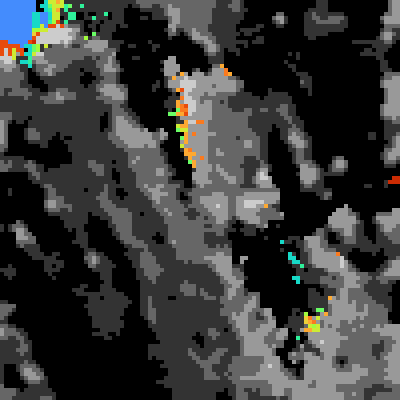
\includegraphics[width=0.32\linewidth]{img/experimentacion/naturales/Flame3/comparacion/flame_plot_1/paso30s_9x9_2x32_420s.png}
			\caption{30 s, $9 \times 9$, 2:32}
			\label{fig:flame_comparacion1_paso30s_9x9_2x32}
		\end{subfigure}
		\\[6pt]
		\begin{subfigure}[t]{0.48\textwidth}
			\centering
			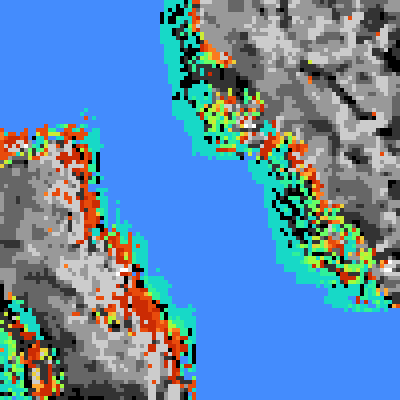
\includegraphics[width=0.32\linewidth]{img/experimentacion/naturales/Flame3/comparacion/flame_plot_1/paso30s_9x9_3x64_150s.png}\hfill
			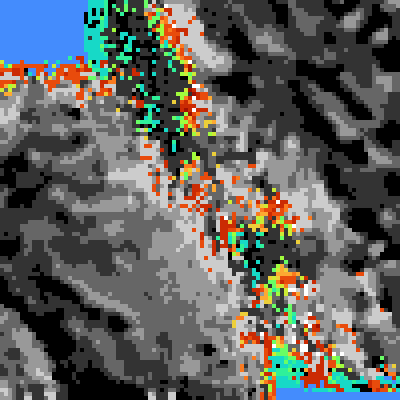
\includegraphics[width=0.32\linewidth]{img/experimentacion/naturales/Flame3/comparacion/flame_plot_1/paso30s_9x9_3x64_300s.png}\hfill
			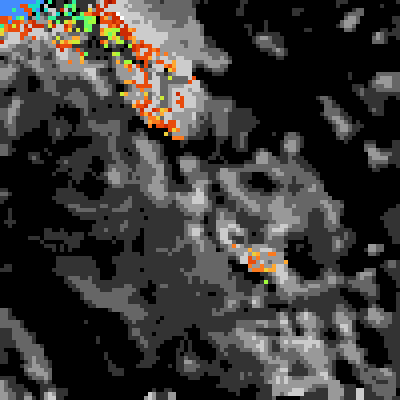
\includegraphics[width=0.32\linewidth]{img/experimentacion/naturales/Flame3/comparacion/flame_plot_1/paso30s_9x9_3x64_420s.png}
			\caption{30 s, $9 \times 9$, 3:64}
			\label{fig:flame_comparacion1_paso30s_9x9_3x64}
		\end{subfigure}
		\hfill
		\begin{subfigure}[t]{0.48\textwidth}
			\centering
			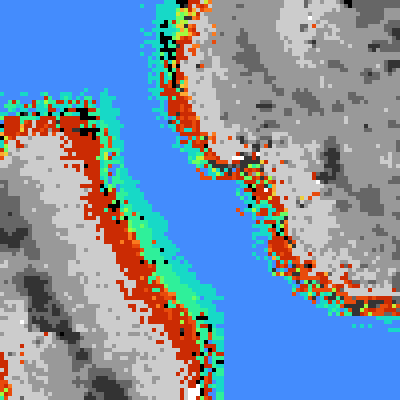
\includegraphics[width=0.32\linewidth]{img/experimentacion/naturales/Flame3/comparacion/flame_plot_1/paso30s_dispersa41_3x64_150s.png}\hfill
			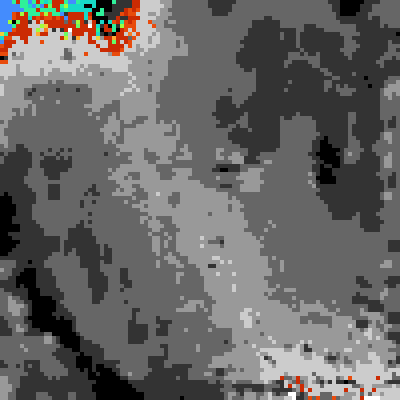
\includegraphics[width=0.32\linewidth]{img/experimentacion/naturales/Flame3/comparacion/flame_plot_1/paso30s_dispersa41_3x64_300s.png}\hfill
			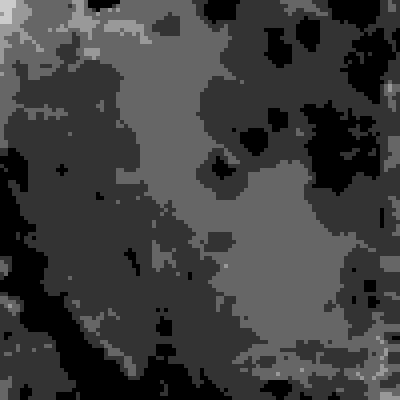
\includegraphics[width=0.32\linewidth]{img/experimentacion/naturales/Flame3/comparacion/flame_plot_1/paso30s_dispersa41_3x64_420s.png}
			\caption{30 s, dispersa, 3:64}
			\label{fig:flame_comparacion1_paso30s_dispersa41_3x64}
		\end{subfigure}
		\\[6pt]
		\begin{subfigure}[t]{0.48\textwidth}
			\centering
			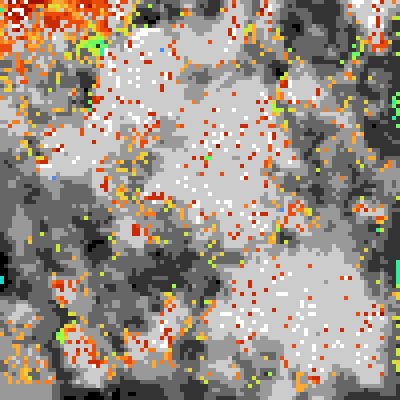
\includegraphics[width=0.32\linewidth]{img/experimentacion/naturales/Flame3/comparacion/flame_plot_1/paso5s_9x9_4x256_150s.png}\hfill
			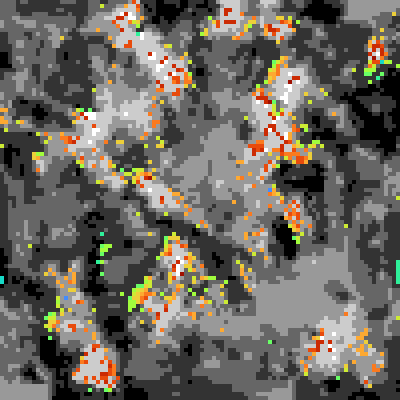
\includegraphics[width=0.32\linewidth]{img/experimentacion/naturales/Flame3/comparacion/flame_plot_1/paso5s_9x9_4x256_300s.png}\hfill
			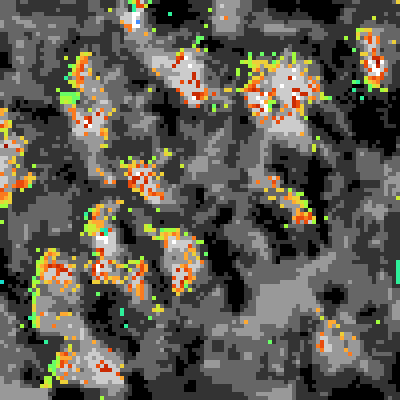
\includegraphics[width=0.32\linewidth]{img/experimentacion/naturales/Flame3/comparacion/flame_plot_1/paso5s_9x9_4x256_420s.png}
			\caption{5 s, $9 \times 9$, 4:256}
			\label{fig:flame_comparacion1_paso5s_9x9_4x256}
		\end{subfigure}
		\hfill
		\begin{subfigure}[t]{0.48\textwidth}
			\centering
			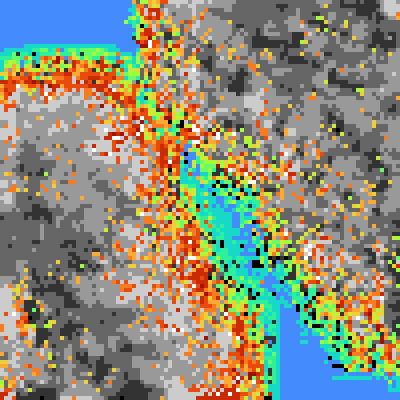
\includegraphics[width=0.32\linewidth]{img/experimentacion/naturales/Flame3/comparacion/flame_plot_1/paso15s_9x9_4x256_150s.png}\hfill
			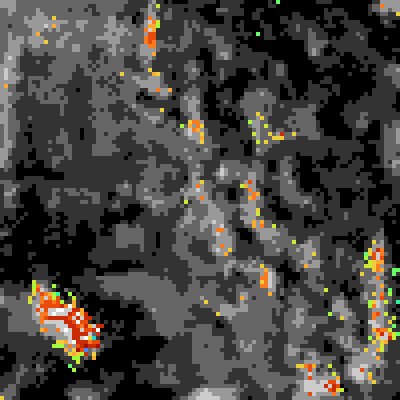
\includegraphics[width=0.32\linewidth]{img/experimentacion/naturales/Flame3/comparacion/flame_plot_1/paso15s_9x9_4x256_300s.png}\hfill
			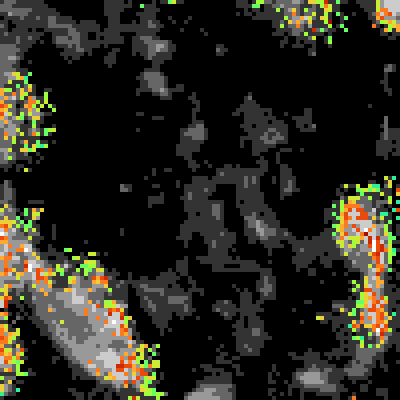
\includegraphics[width=0.32\linewidth]{img/experimentacion/naturales/Flame3/comparacion/flame_plot_1/paso15s_9x9_4x256_420s.png}
			\caption{15 s, $9 \times 9$, 4:256}
			\label{fig:flame_comparacion1_paso15s_9x9_4x256}
		\end{subfigure}
		\leyendaflame
		\caption{Evolución de flame\_plot\_1 (a) y simulación libre de las 9 configuraciones de ambas pruebas, entrenadas con flame\_plot\_2. En cada una: 150, 300 y 420 s después de la imagen inicial.}
		\label{fig:flame_comparacion1}
	\end{figure}

	\begin{figure}[htbp]
		\centering
		\begin{subfigure}[t]{0.48\textwidth}
			\centering
			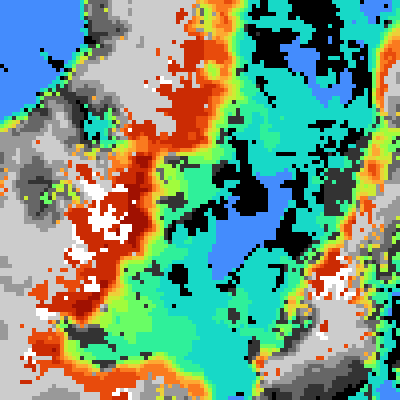
\includegraphics[width=0.32\linewidth]{img/experimentacion/naturales/Flame3/comparacion/flame_plot_2/real_90s.png}\hfill
			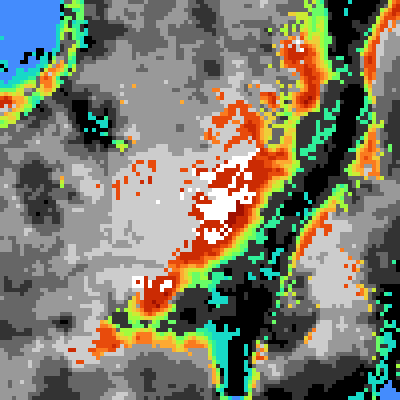
\includegraphics[width=0.32\linewidth]{img/experimentacion/naturales/Flame3/comparacion/flame_plot_2/real_150s.png}\hfill
			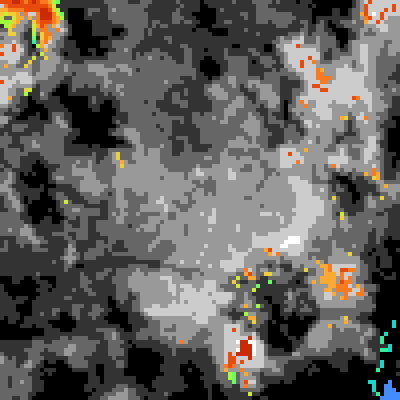
\includegraphics[width=0.32\linewidth]{img/experimentacion/naturales/Flame3/comparacion/flame_plot_2/real_240s.png}
			\caption{Real}
			\label{fig:flame_comparacion2_real}
		\end{subfigure}
		\hfill
		\begin{subfigure}[t]{0.48\textwidth}
			\centering
			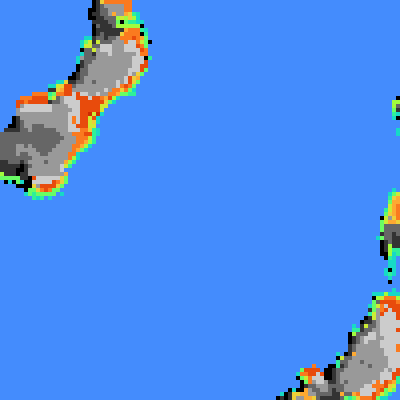
\includegraphics[width=0.32\linewidth]{img/experimentacion/naturales/Flame3/comparacion/flame_plot_2/paso15s_9x9_2x32_90s.png}\hfill
			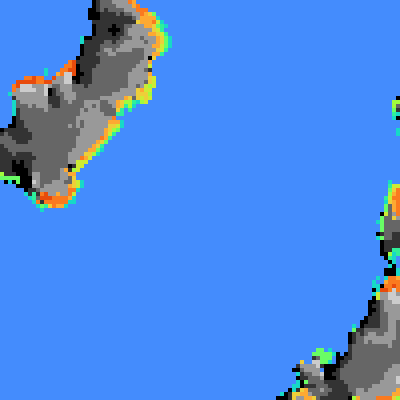
\includegraphics[width=0.32\linewidth]{img/experimentacion/naturales/Flame3/comparacion/flame_plot_2/paso15s_9x9_2x32_150s.png}\hfill
			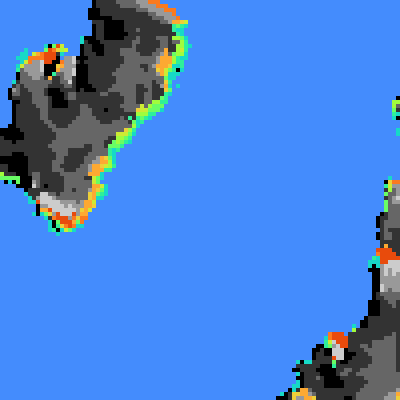
\includegraphics[width=0.32\linewidth]{img/experimentacion/naturales/Flame3/comparacion/flame_plot_2/paso15s_9x9_2x32_240s.png}
			\caption{15 s, $9 \times 9$, 2:32}
			\label{fig:flame_comparacion2_paso15s_9x9_2x32}
		\end{subfigure}
		\\[6pt]
		\begin{subfigure}[t]{0.48\textwidth}
			\centering
			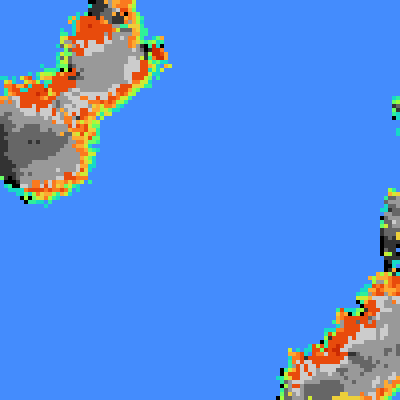
\includegraphics[width=0.32\linewidth]{img/experimentacion/naturales/Flame3/comparacion/flame_plot_2/paso15s_9x9_3x64_90s.png}\hfill
			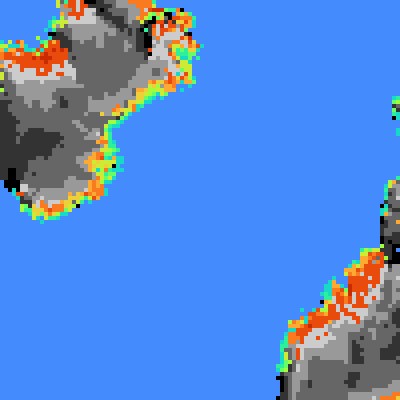
\includegraphics[width=0.32\linewidth]{img/experimentacion/naturales/Flame3/comparacion/flame_plot_2/paso15s_9x9_3x64_150s.png}\hfill
			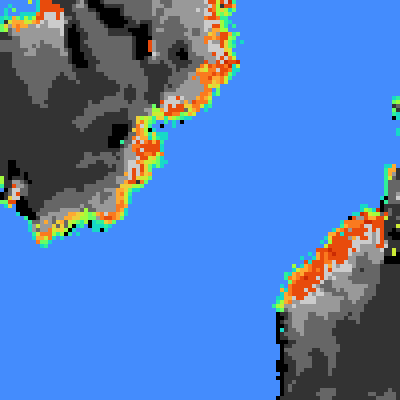
\includegraphics[width=0.32\linewidth]{img/experimentacion/naturales/Flame3/comparacion/flame_plot_2/paso15s_9x9_3x64_240s.png}
			\caption{15 s, $9 \times 9$, 3:64}
			\label{fig:flame_comparacion2_paso15s_9x9_3x64}
		\end{subfigure}
		\hfill
		\begin{subfigure}[t]{0.48\textwidth}
			\centering
			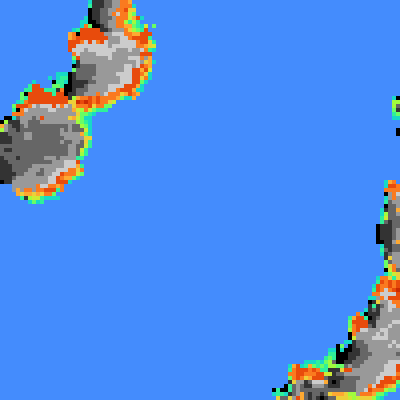
\includegraphics[width=0.32\linewidth]{img/experimentacion/naturales/Flame3/comparacion/flame_plot_2/paso15s_dispersa41_3x64_90s.png}\hfill
			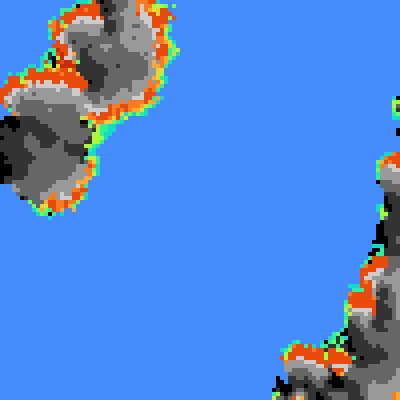
\includegraphics[width=0.32\linewidth]{img/experimentacion/naturales/Flame3/comparacion/flame_plot_2/paso15s_dispersa41_3x64_150s.png}\hfill
			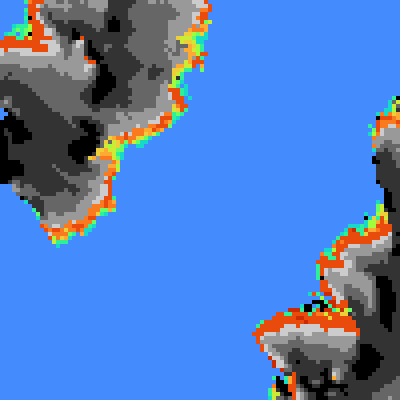
\includegraphics[width=0.32\linewidth]{img/experimentacion/naturales/Flame3/comparacion/flame_plot_2/paso15s_dispersa41_3x64_240s.png}
			\caption{15 s, dispersa, 3:64}
			\label{fig:flame_comparacion2_paso15s_dispersa41_3x64}
		\end{subfigure}
		\\[6pt]
		\begin{subfigure}[t]{0.48\textwidth}
			\centering
			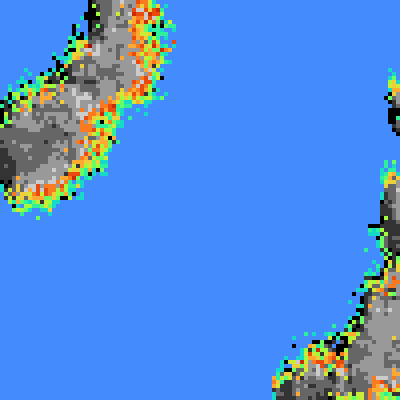
\includegraphics[width=0.32\linewidth]{img/experimentacion/naturales/Flame3/comparacion/flame_plot_2/paso15s_dispersa41_4x256_90s.png}\hfill
			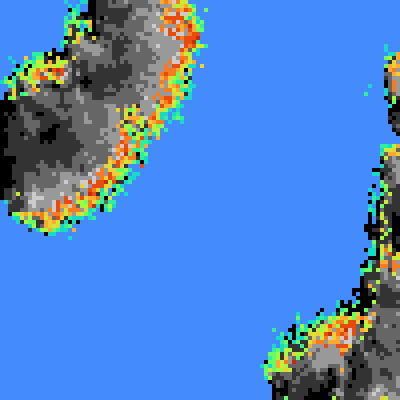
\includegraphics[width=0.32\linewidth]{img/experimentacion/naturales/Flame3/comparacion/flame_plot_2/paso15s_dispersa41_4x256_150s.png}\hfill
			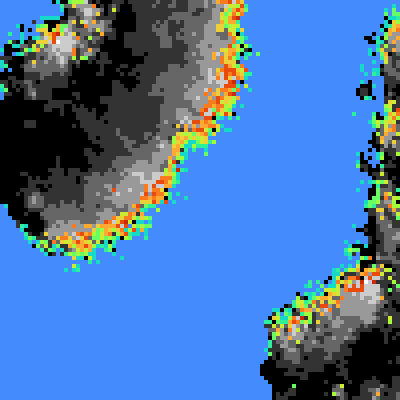
\includegraphics[width=0.32\linewidth]{img/experimentacion/naturales/Flame3/comparacion/flame_plot_2/paso15s_dispersa41_4x256_240s.png}
			\caption{15 s, dispersa, 4:256}
			\label{fig:flame_comparacion2_paso15s_dispersa41_4x256}
		\end{subfigure}
		\hfill
		\begin{subfigure}[t]{0.48\textwidth}
			\centering
			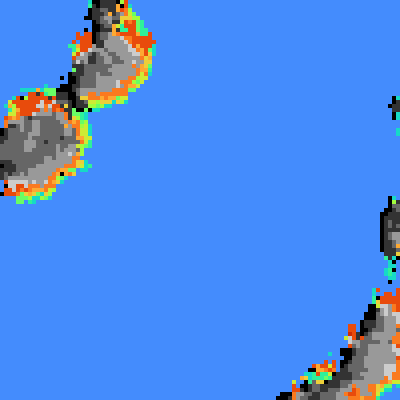
\includegraphics[width=0.32\linewidth]{img/experimentacion/naturales/Flame3/comparacion/flame_plot_2/paso30s_9x9_2x32_90s.png}\hfill
			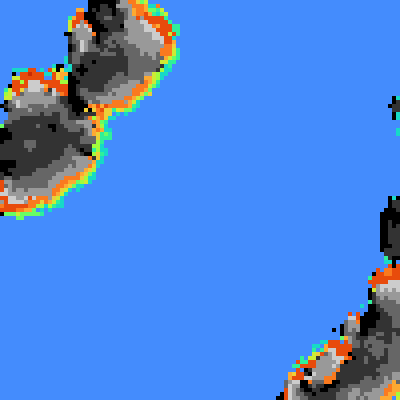
\includegraphics[width=0.32\linewidth]{img/experimentacion/naturales/Flame3/comparacion/flame_plot_2/paso30s_9x9_2x32_150s.png}\hfill
			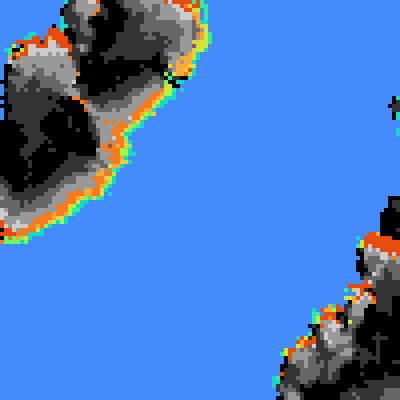
\includegraphics[width=0.32\linewidth]{img/experimentacion/naturales/Flame3/comparacion/flame_plot_2/paso30s_9x9_2x32_240s.png}
			\caption{30 s, $9 \times 9$, 2:32}
			\label{fig:flame_comparacion2_paso30s_9x9_2x32}
		\end{subfigure}
		\\[6pt]
		\begin{subfigure}[t]{0.48\textwidth}
			\centering
			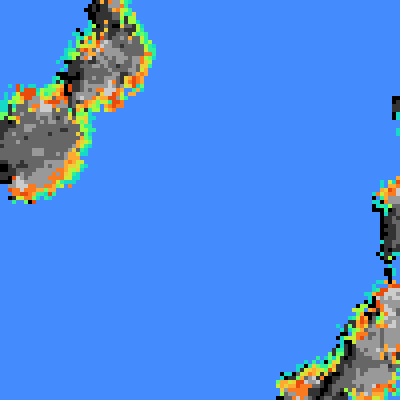
\includegraphics[width=0.32\linewidth]{img/experimentacion/naturales/Flame3/comparacion/flame_plot_2/paso30s_9x9_3x64_90s.png}\hfill
			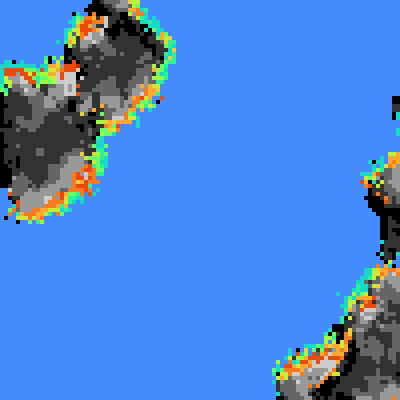
\includegraphics[width=0.32\linewidth]{img/experimentacion/naturales/Flame3/comparacion/flame_plot_2/paso30s_9x9_3x64_150s.png}\hfill
			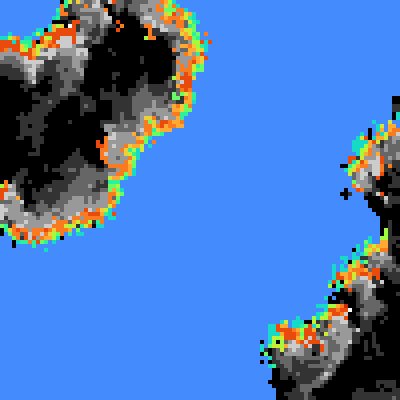
\includegraphics[width=0.32\linewidth]{img/experimentacion/naturales/Flame3/comparacion/flame_plot_2/paso30s_9x9_3x64_240s.png}
			\caption{30 s, $9 \times 9$, 3:64}
			\label{fig:flame_comparacion2_paso30s_9x9_3x64}
		\end{subfigure}
		\hfill
		\begin{subfigure}[t]{0.48\textwidth}
			\centering
			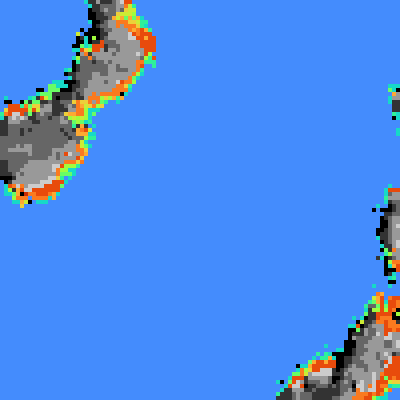
\includegraphics[width=0.32\linewidth]{img/experimentacion/naturales/Flame3/comparacion/flame_plot_2/paso30s_dispersa41_3x64_90s.png}\hfill
			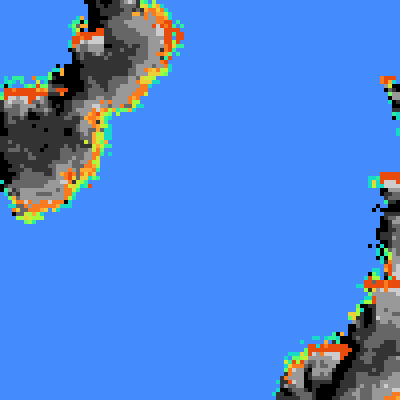
\includegraphics[width=0.32\linewidth]{img/experimentacion/naturales/Flame3/comparacion/flame_plot_2/paso30s_dispersa41_3x64_150s.png}\hfill
			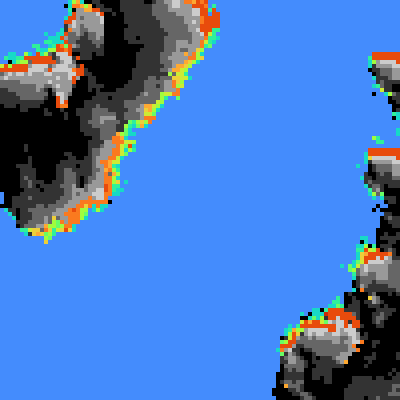
\includegraphics[width=0.32\linewidth]{img/experimentacion/naturales/Flame3/comparacion/flame_plot_2/paso30s_dispersa41_3x64_240s.png}
			\caption{30 s, dispersa, 3:64}
			\label{fig:flame_comparacion2_paso30s_dispersa41_3x64}
		\end{subfigure}
		\\[6pt]
		\begin{subfigure}[t]{0.48\textwidth}
			\centering
			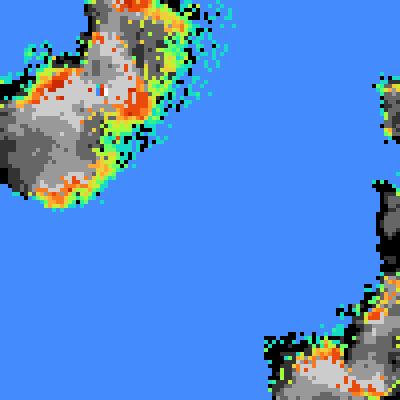
\includegraphics[width=0.32\linewidth]{img/experimentacion/naturales/Flame3/comparacion/flame_plot_2/paso5s_9x9_4x256_90s.png}\hfill
			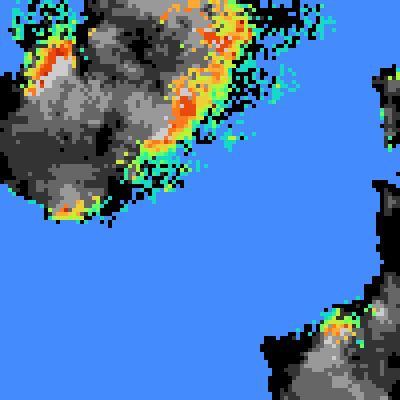
\includegraphics[width=0.32\linewidth]{img/experimentacion/naturales/Flame3/comparacion/flame_plot_2/paso5s_9x9_4x256_150s.png}\hfill
			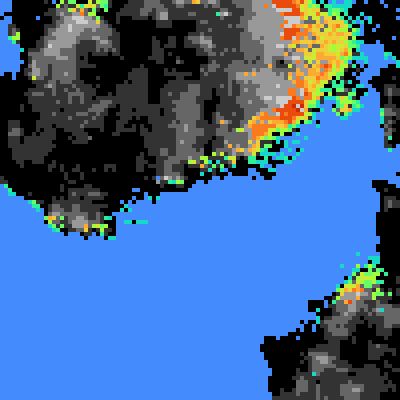
\includegraphics[width=0.32\linewidth]{img/experimentacion/naturales/Flame3/comparacion/flame_plot_2/paso5s_9x9_4x256_240s.png}
			\caption{5 s, $9 \times 9$, 4:256}
			\label{fig:flame_comparacion2_paso5s_9x9_4x256}
		\end{subfigure}
		\hfill
		\begin{subfigure}[t]{0.48\textwidth}
			\centering
			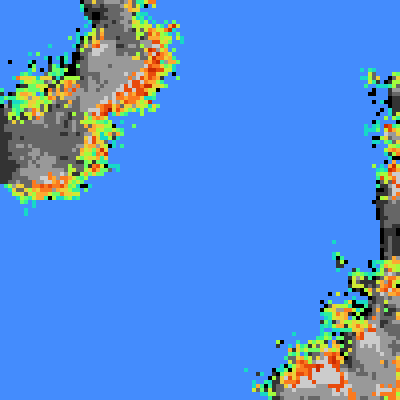
\includegraphics[width=0.32\linewidth]{img/experimentacion/naturales/Flame3/comparacion/flame_plot_2/paso15s_9x9_4x256_90s.png}\hfill
			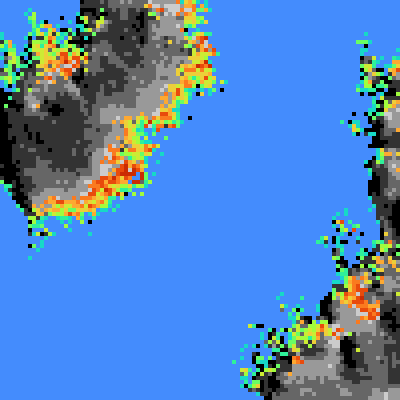
\includegraphics[width=0.32\linewidth]{img/experimentacion/naturales/Flame3/comparacion/flame_plot_2/paso15s_9x9_4x256_150s.png}\hfill
			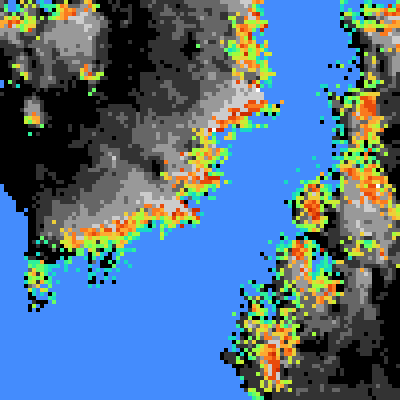
\includegraphics[width=0.32\linewidth]{img/experimentacion/naturales/Flame3/comparacion/flame_plot_2/paso15s_9x9_4x256_240s.png}
			\caption{15 s, $9 \times 9$, 4:256}
			\label{fig:flame_comparacion2_paso15s_9x9_4x256}
		\end{subfigure}
		\leyendaflame
		\caption{Evolución de flame\_plot\_2 (a) y simulación libre de las 9 configuraciones de ambas pruebas, entrenadas con flame\_plot\_1. En cada una: 90, 150 y 240 s después de la imagen inicial.}
		\label{fig:flame_comparacion2}
	\end{figure}
		
	Este experimento está limitado por varias razones. La primera es la cantidad de información recopilada, ya que FLAME~3 es uno de los pocos conjuntos de datos que registran la propagación del fuego, y específicamente con vista cenital. Además, este experimento no contempla todas las variables del sistema: únicamente se utilizan células en un plano bidimensional, sin considerar otras variables como la altura, las carreteras, los árboles, la dirección del viento o la humedad, que cambian drásticamente la dinámica.

	La reducción del conjunto de datos a únicamente dos muestras no permite generalizar a múltiples escenarios, y aparecen comportamientos diferentes que dependen de la geografía del sistema. Por ejemplo, en flame\_plot\_1 los cambios de temperatura casi siempre ocurren cerca de la línea del fuego, es decir, el sistema se mantiene frío excepto cuando el fuego se aproxima. Por otro lado, en flame\_plot\_2 primero se propagan las temperaturas medias y después son alcanzadas por el fuego.

	Otra consideración fue la dirección de la propagación. Aunque se probó rotar el sistema, las rotaciones añaden ruido, ya que la cámara está orientada hacia el norte y, en ambas pruebas, el viento apunta al este, por lo que las llamas, o las temperaturas, se mueven en esa dirección.

	A diferencia de lo que ocurrió con los sistemas ya conocidos, la red neuronal no tuvo el mismo éxito al intentar replicar el comportamiento. Sin embargo, algunas de las configuraciones sí pueden utilizarse para mostrarlo. En este caso, la selección visual de los experimentos tuvo como objetivo recoger aquellas configuraciones que podrían simular la propagación del fuego y la colisión de diferentes frentes, con una velocidad constante, sin generación espontánea de fuego y sin que un mismo lugar se queme dos veces.

	De este experimento podemos concluir que podría ser posible replicar estos sistemas con la cantidad de información suficiente para generalizarlos a cualquier entorno. Se pudieron diseñar autómatas celulares neuronales que propagan el fuego, pero basados únicamente en el registro de temperaturas y no en la geografía, que aportaría información específica para ayudar al sistema.
	


